% ==============================================================================
% IEEE-Style Two-Column Technical Sign-Off Report (6 Pages, Tight IEEE Layout)
% Project: tt_um_arcadia1_vco_adc (Tiny Tapeout SKY26e, sky130A 1x2 Analog Tile)
% ==============================================================================
\documentclass[10pt,twocolumn,letterpaper]{article}

% --- Fonts & Microtypography (Authentic IEEE Times Roman Look) ---
\usepackage[nott]{newtxtext}
\usepackage{newtxmath}
\renewcommand{\ttdefault}{cmtt}
\usepackage[T1]{fontenc}
\usepackage[utf8]{inputenc}
\usepackage[protrusion=true,expansion=true]{microtype}

% --- Page Geometry (IEEEtran Letter Dimensions) ---
\usepackage[top=0.58in,bottom=0.58in,left=0.56in,right=0.56in,columnsep=0.22in]{geometry}

% --- Graphics, Tables, Floats, Equations ---
\usepackage{graphicx}
\usepackage{booktabs}
\usepackage{multirow}
\usepackage{array}
\usepackage{amsmath}
\usepackage{xcolor}
\usepackage{dblfloatfix}
\usepackage{flushend}
\usepackage{enumitem}
\usepackage{cite}
\usepackage[colorlinks=true,linkcolor=navy,citecolor=navy,urlcolor=navy]{hyperref}

\definecolor{navy}{RGB}{11,60,93}
\definecolor{muted}{RGB}{71,85,105}
\definecolor{okgreen}{RGB}{20,125,100}
\definecolor{warnred}{RGB}{185,28,28}

% --- IEEE Section, Subsection & Caption Formatting ---
\usepackage{titlesec}
\renewcommand{\thesection}{\Roman{section}}
\renewcommand{\thesubsection}{\Alph{subsection}}
\renewcommand{\thetable}{\Roman{table}}

\titleformat{\section}{\centering\scshape\normalsize}{\thesection.}{0.5em}{}
\titlespacing*{\section}{0pt}{7pt plus 1.5pt minus 1pt}{3pt plus 0.5pt}
\titleformat{\subsection}{\itshape\normalsize}{\thesubsection.}{0.45em}{}
\titlespacing*{\subsection}{0pt}{5pt plus 1pt minus 0.5pt}{1.5pt plus 0.5pt}

\usepackage{caption}
\usepackage{subcaption}
\captionsetup[figure]{font=footnotesize,labelfont=bf,labelsep=period,name=Fig.,skip=2.5pt}
\captionsetup[table]{font={footnotesize,sc},labelfont=sc,labelsep=newline,justification=centering,name=TABLE,skip=2.5pt}
\captionsetup[subfigure]{font=scriptsize,skip=1pt}

% --- Running Header & Footer ---
\usepackage{fancyhdr}
\pagestyle{fancy}
\fancyhf{}
\fancyhead[L]{\scriptsize\textsc{Tiny Tapeout SKY26e Technical Report --- \textup{\texttt{tt\_um\_arcadia1\_vco\_adc}}}}
\fancyhead[R]{\scriptsize\thepage}
\renewcommand{\headrulewidth}{0.4pt}
\fancypagestyle{firstpage}{
  \fancyhf{}
  \fancyfoot[C]{\scriptsize\thepage}
  \renewcommand{\headrulewidth}{0pt}
}

% --- Compact Float & Table Tuning for Crisp 6-Page IEEE Pagination ---
\renewcommand{\topfraction}{0.92}
\renewcommand{\bottomfraction}{0.88}
\renewcommand{\textfraction}{0.06}
\renewcommand{\floatpagefraction}{0.82}
\renewcommand{\dbltopfraction}{0.92}
\renewcommand{\dblfloatpagefraction}{0.82}
\setlength{\textfloatsep}{6pt plus 1.5pt minus 1.5pt}
\setlength{\dbltextfloatsep}{6pt plus 1.5pt minus 1.5pt}
\setlength{\floatsep}{5pt plus 1pt minus 1pt}
\setlength{\intextsep}{5pt plus 1pt minus 1pt}
\renewcommand{\arraystretch}{1.07}

% ==============================================================================
% POST-LAYOUT FULL-TRANSISTOR FLAT PEX TONE MACROS (nesthorn Step 5A, 6/6 PASS)
% Extracted V2_03 C-only flat PEX (1,248 BSIM4/PDK devices, 2,443 parasitic caps,
% 16 x 1 pF pin loads, N=2048, fin=14.65 kHz, HD3=43.95 kHz in-band, tmax=0.5 ns)
% ==============================================================================
\newcommand{\pexTTsndr}{$70.1$}     \newcommand{\pexTThdTwo}{$-77.8$}    \newcommand{\pexTThdThree}{$-71.9$}    \newcommand{\pexTTidd}{$173.5$}
\newcommand{\pexSSsndr}{$69.0$}     \newcommand{\pexSShdTwo}{$-77.4$}    \newcommand{\pexSShdThree}{$-70.4$}    \newcommand{\pexSSidd}{$176.1$}
\newcommand{\pexFFsndr}{$69.3$}     \newcommand{\pexFFhdTwo}{$-76.8$}    \newcommand{\pexFFhdThree}{$-70.7$}    \newcommand{\pexFFidd}{$173.2$}
\newcommand{\pexSFsndr}{$69.3$}     \newcommand{\pexSFhdTwo}{$-76.8$}    \newcommand{\pexSFhdThree}{$-70.5$}    \newcommand{\pexSFidd}{$177.1$}
\newcommand{\pexFSsndr}{$70.6$}     \newcommand{\pexFShdTwo}{$-76.9$}    \newcommand{\pexFShdThree}{$-72.5$}    \newcommand{\pexFSidd}{$170.9$}
\newcommand{\pexFSLLsndr}{$70.4$}   \newcommand{\pexFSLLhdTwo}{$-76.9$}  \newcommand{\pexFSLLhdThree}{$-72.5$}  \newcommand{\pexFSLLidd}{$175.4$}

\begin{document}
\thispagestyle{firstpage}

% --- Full-Width IEEE Title, Author, Abstract & Index Terms ---
\twocolumn[{%
\begin{center}
  {\LARGE\bfseries A 1.8-V Pseudo-Differential Second-Order Closed-Loop VCO $\Delta\Sigma$ ADC with Brick-Wall Active Clamp and Isolated Digital Feedback in 130-nm CMOS\par}
  \vspace{5pt}
  {\normalsize Arcadia-1 Analog Design Team\par}
  \vspace{1.5pt}
  {\footnotesize\itshape Open-Source Silicon Tapeout: Tiny Tapeout SKY26e (\textup{\texttt{sky130A}} 130-nm CMOS, $1\times2$ Analog Tile \textup{\texttt{tt\_um\_arcadia1\_vco\_adc}}, $161.0 \times 225.76\,\mu\text{m}^2$)\par}
\end{center}
\vspace{3pt}
\begin{quote}
\small
\textbf{\textit{Abstract}---This report presents the design, verification, and physical sign-off of \textup{\texttt{tt\_um\_arcadia1\_vco\_adc}}, a 1.8-V pseudo-differential second-order continuous-time closed-loop VCO $\Delta\Sigma$ ADC in \textup{\texttt{sky130A}} ($161.0\times225.76\,\mu\text{m}^2$ Tiny Tapeout $1\times2$ tile, $f_s=10\text{ MHz}$, $\text{BW}=50\text{ kHz}$, $\text{OSR}=100$, $\pm0.60\text{ V}$ diff. full scale around $0.90\text{ V}$). Each half cascades a common-centroid 5T OTA-C integrator with a 7-stage current-starved ring VCO, two-rank XOR phase differentiator, and intrinsically barrel-shifted 7-element NRZ RDAC. Three upgrades over S13 eliminate key silicon risks: (1)~upsizing the OTA ($48/3\,\mu\text{m}$ NMOS, $16/2\,\mu\text{m}$ PMOS, $23\,\mu\text{A}$ tail) lowers BSIM4 $1/f+$thermal noise by $+10.2\text{ dB}$ ($74.6\to22.9\,\mu\text{V}_{\text{rms}}$, $79.3\text{ dB}$ ceiling, $85.3\text{ dB}$ FS DR, Tian $\text{PM}=72.2^\circ$); (2)~a zero-static-power 5-FET Miller-compensated active clamp (\textup{\texttt{CLAMP\_A5}}, $14.3$--$48.9\text{ nA}$ @ $1.15\text{ V}$, $0.00\text{ dB}$ noise/HD3 penalty) hard-limits $f_{\text{VCO}}\le6.66\text{ MHz}$ below $7.5\text{ MHz}$ aliasing latch-up; and (3)~dedicated \textup{\texttt{buf\_4}} pin buffers cut BSIM4 XOR glitch charge theft $19\times$--$90\times$ and rise/fall asymmetry $20\times$--$215\times$ over $C_{\text{load}}=1$--$5\text{ pF}$. True in-band $14.65\text{ kHz}$ ($\text{HD3}=43.95\text{ kHz}$ in-band) sign-off achieves $71.8\text{ dB}$ TT schematic SNDR ($68.5$--$73.4\text{ dB}$ across 17 $1.80/1.98\text{ V}$ PVT+R/C corners; $71.1\text{ dB}$ median across 16 \textup{\texttt{tt\_mm}} MC seeds) and \textbf{$69.0$--$70.6\text{ dB}$ SNDR} ($77.7$--$81.9\text{ dB}$ SNR, $\text{HD3}=-70.4$ to $-72.5\text{ dBc}$) across all 6 full-transistor flat-PEX corners ($173.4\,\mu\text{W}$ core / $312\,\mu\text{W}$ PEX w/ $16\times1\text{ pF}$), with 0 DRC, unique LVS ($54/54$ pins), 16/16 TT precheck, and 4/4 flat-PEX latch-up stress passes.}

\vspace{2pt}
\textbf{\textit{Index Terms}---Continuous-time $\Delta\Sigma$ ADC, VCO-based quantizer, second-order noise shaping, active Miller clamp, digital output isolation, \textup{\texttt{sky130A}}, Tiny Tapeout.}
\end{quote}
\vspace{2pt}
}]

% ==============================================================================
\section{Introduction}
% ==============================================================================
Voltage-controlled oscillator (VCO)-based analog-to-digital converters replace power-hungry comparators and precision multibit DACs with compact, time-domain phase quantizers that naturally scale with CMOS technology~\cite{straayer2008,taylor2010}. Operated open-loop, however, a ring oscillator exhibits severe static $f_{\text{VCO}}(V_{\text{ctrl}})$ nonlinearity that limits distortion to $40$--$50\text{ dB}$. Embedding the ring VCO inside a continuous-time negative-feedback loop preceded by an active OTA-C integrator solves both problems: loop gain suppresses VCO nonlinearity in-band, the cascade of integrator and VCO phase integration yields true second-order ($40\text{ dB/dec}$) noise shaping, and sampling all $M=7$ ring phases provides a 7-level quantizer whose phase rotation implements first-order intrinsic dynamic element matching (DEM) across the resistor DAC~\cite{straayer2008,xing2015}.

This work implements a pseudo-differential second-order closed-loop VCO $\Delta\Sigma$ ADC (\texttt{tt\_um\_arcadia1\_vco\_adc}) within a Tiny Tapeout SKY26e $1\times2$ analog tile ($161.0\times225.76\,\mu\text{m}^2$, single $1.8\text{ V}$ supply \texttt{VDPWR}, analog inputs \texttt{ua[0:1]}, digital outputs \texttt{uo\_out[7:0]} and \texttt{uio\_out[7:0]}). Deep verification of the initial baseline layout (\texttt{Base\_S13}) revealed three latent silicon risks masked by nominal noiseless transient simulations:
\begin{enumerate}[leftmargin=1.3em,itemsep=1pt,topsep=1.5pt]
  \item \textbf{OTA $1/f$ Noise Ceiling:} A compact $8/1\,\mu\text{m}$ input pair produced $74.6\,\mu\text{V}_{\text{rms}}$ BSIM4 noise ($100\text{ Hz}$--$50\text{ kHz}$), capping real silicon SNR at $69.1\text{ dB}$ despite $75$--$81\text{ dB}$ noiseless FFTs.
  \item \textbf{Phase-Aliasing Latch-Up ($f_{\text{VCO}}>0.75 f_s$):} During unreset startup or rail overload at fast-NMOS/low-$R$ high-$V_{DD}$ corners (\texttt{fs\_ll}/$1.98\text{ V}$, \texttt{ss\_ll}/$85^\circ\text{C}/1.98\text{ V}$), $v_{\text{ctrl}}$ saturated toward $V_{DD}$, driving $f_{\text{VCO}}$ to $7.85$--$9.33\text{ MHz}$. Above $0.75 f_s=7.5\text{ MHz}$, XOR differentiation aliases backward and inverts feedback polarity, permanently latching the ring near $8.5\text{ MHz}$.
  \item \textbf{External Load Coupling into Feedback DAC:} Driving external $1$--$5\text{ pF}$ pad/mux capacitance directly from first-rank \texttt{dfxtp\_4} skewed \texttt{Q1} vs. \texttt{Q2} at \texttt{xor2\_1}, causing full-rail glitches that stole up to $14.8\text{ ns}$ of DAC charge and injected $6.0\text{ ns}$ rise/fall asymmetry.
\end{enumerate}

The finalized \texttt{V2\_A5} revision resolves all three vulnerabilities with zero clamping static power and complete physical sign-off. Table~\ref{tab:spec} summarizes the specifications and verified gains over \texttt{Base\_S13}.

% --- FIG. 1: Four-Panel Complete Circuit Architecture (Page 2 Top) ---
\begin{figure*}[t]
\centering
\begin{subfigure}[b]{0.26\textwidth}
  \centering
  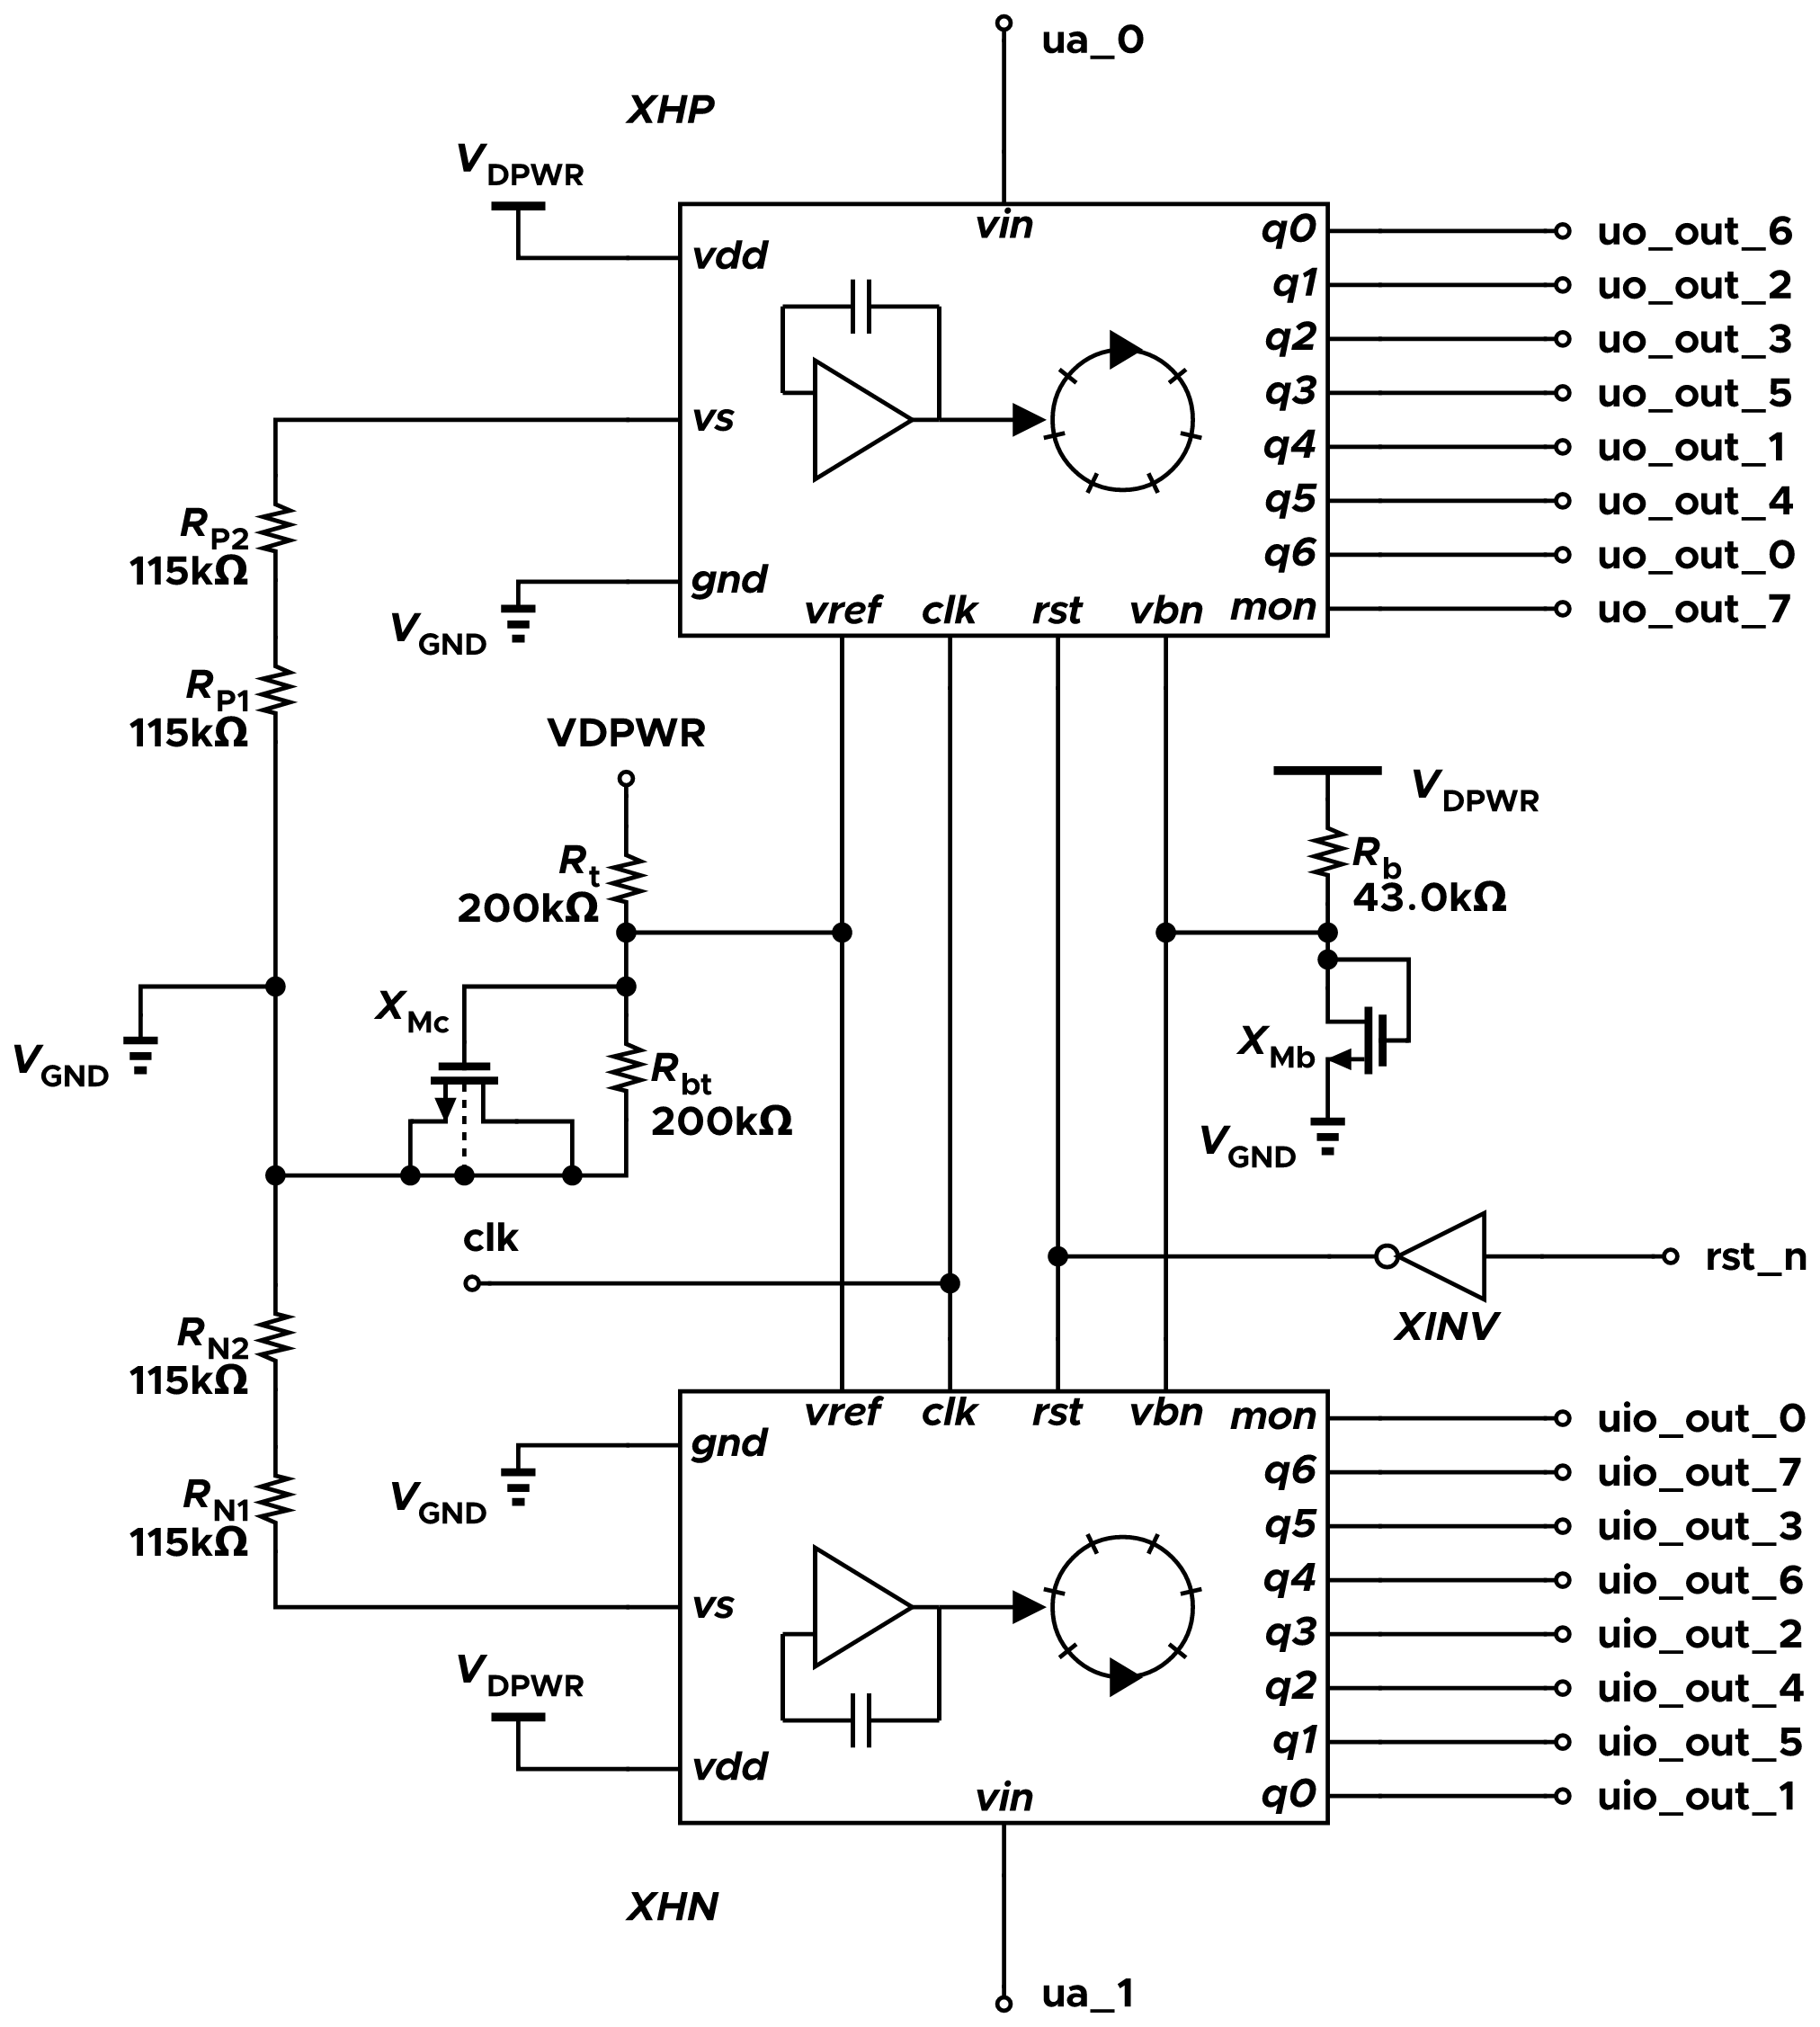
\includegraphics[width=\linewidth]{figs/sch_top.png}
  \caption{Top-level pseudo-differential tile.}
  \label{fig:sch_top}
\end{subfigure}\hfill
\begin{subfigure}[b]{0.57\textwidth}
  \centering
  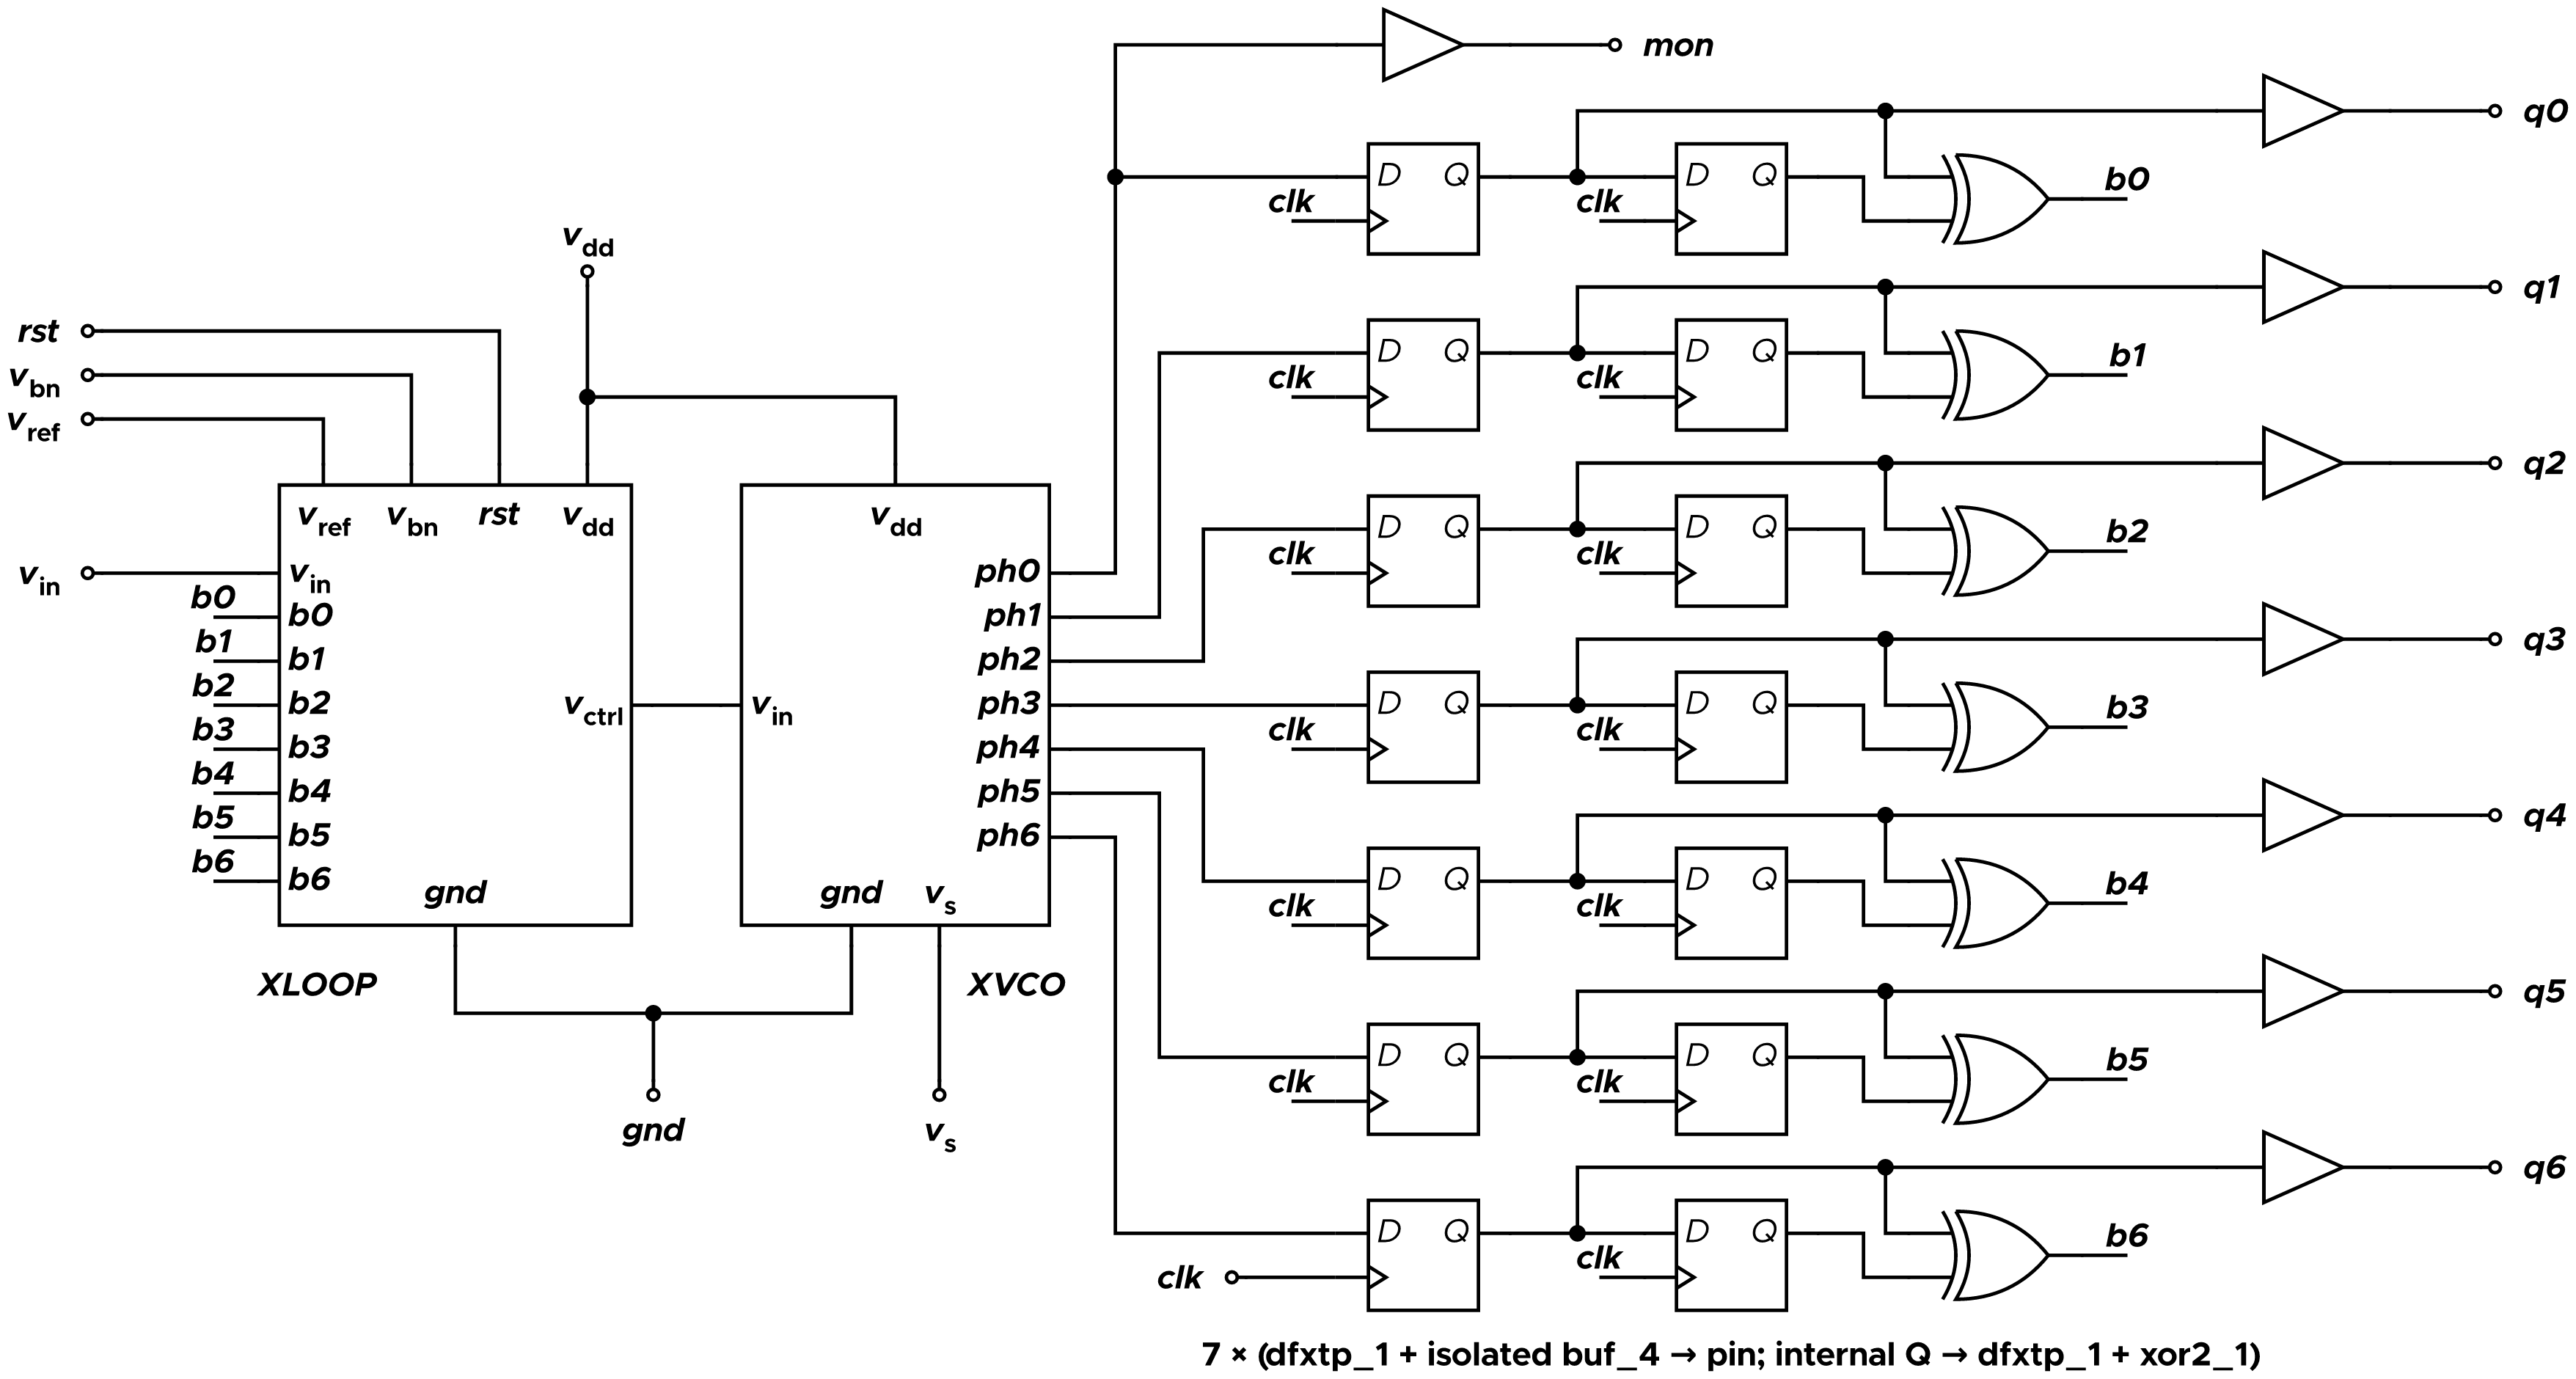
\includegraphics[width=\linewidth]{figs/sch_half.png}
  \caption{One half-channel: loop, 7-stage VCO, and isolated digital backend (\textup{\texttt{dfxtp\_1}} + \textup{\texttt{buf\_4}}).}
  \label{fig:sch_half}
\end{subfigure}
\vspace{1.5pt}

\begin{subfigure}[b]{0.28\textwidth}
  \centering
  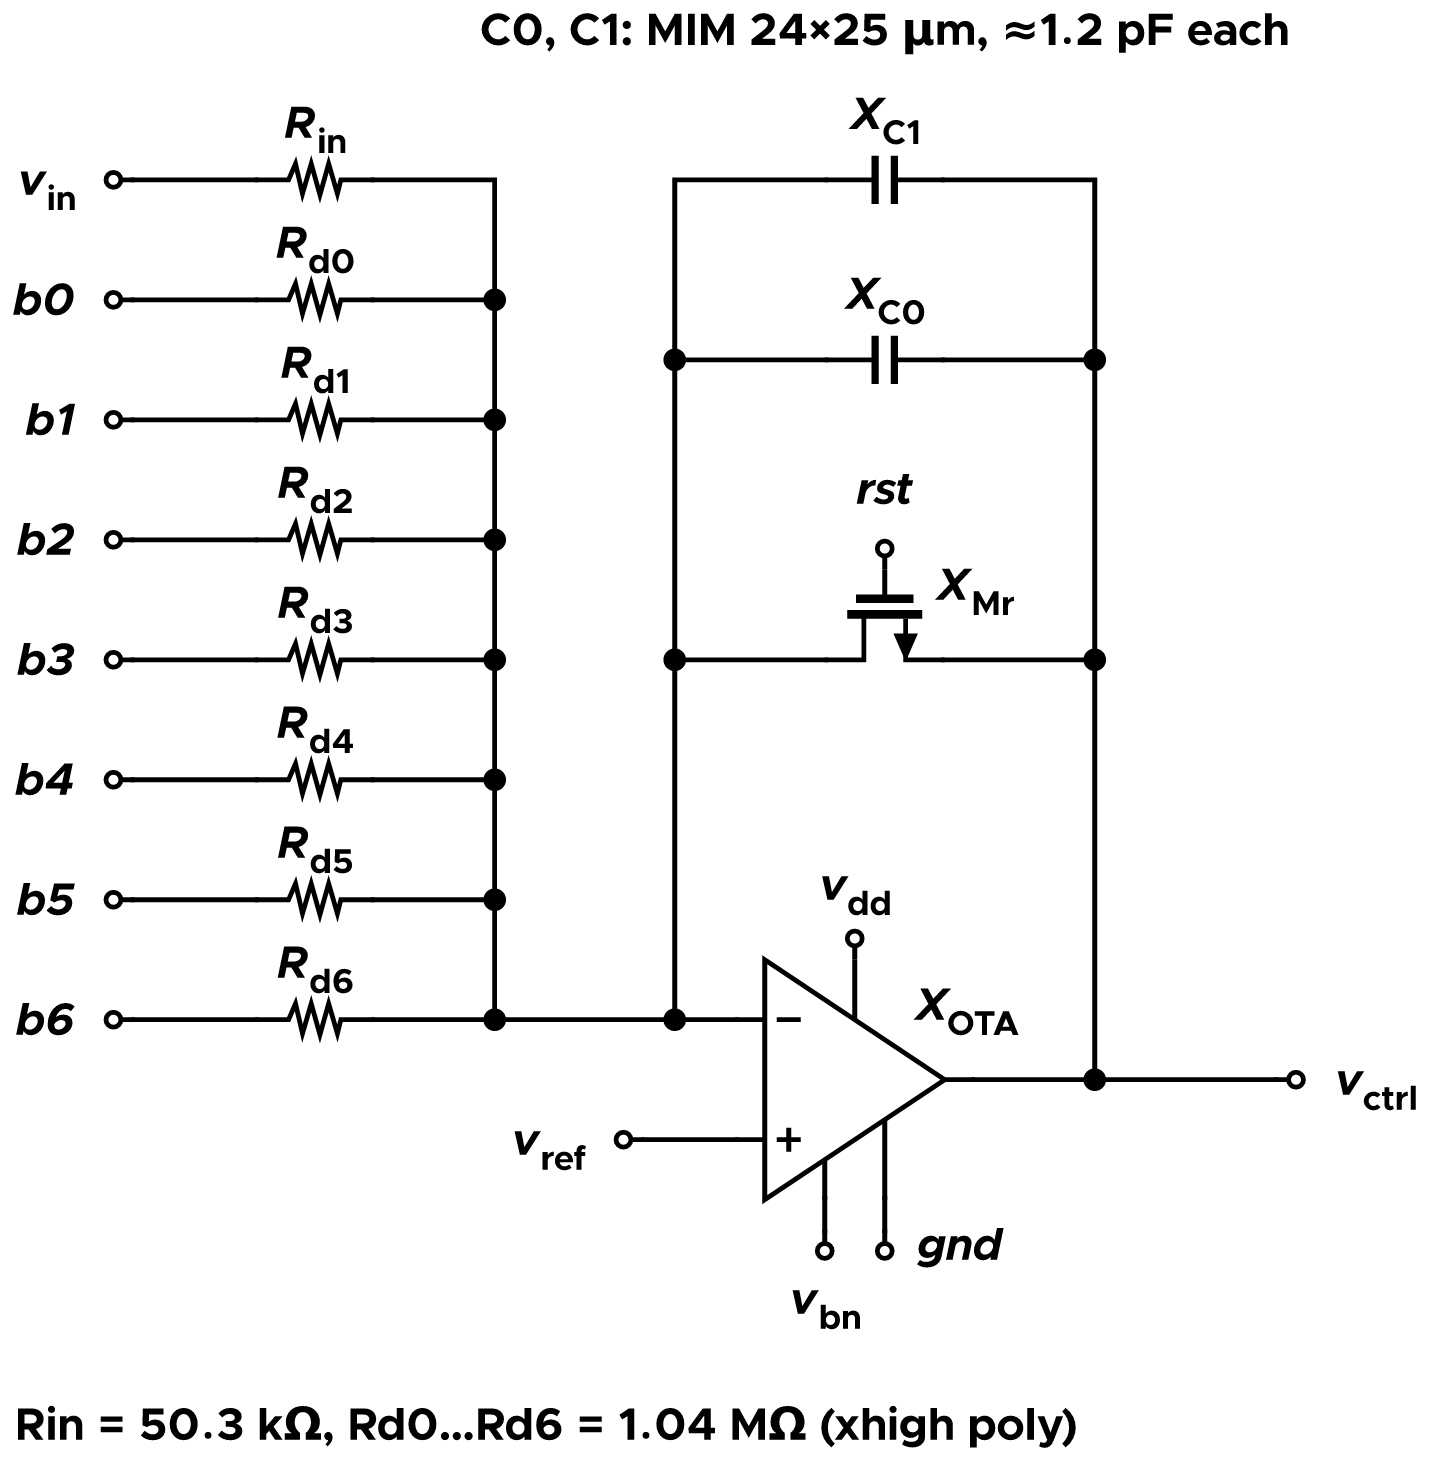
\includegraphics[width=\linewidth]{figs/sch_loop.png}
  \caption{OTA-C integrator \& 7-element RDAC.}
  \label{fig:sch_loop}
\end{subfigure}\hfill
\begin{subfigure}[b]{0.55\textwidth}
  \centering
  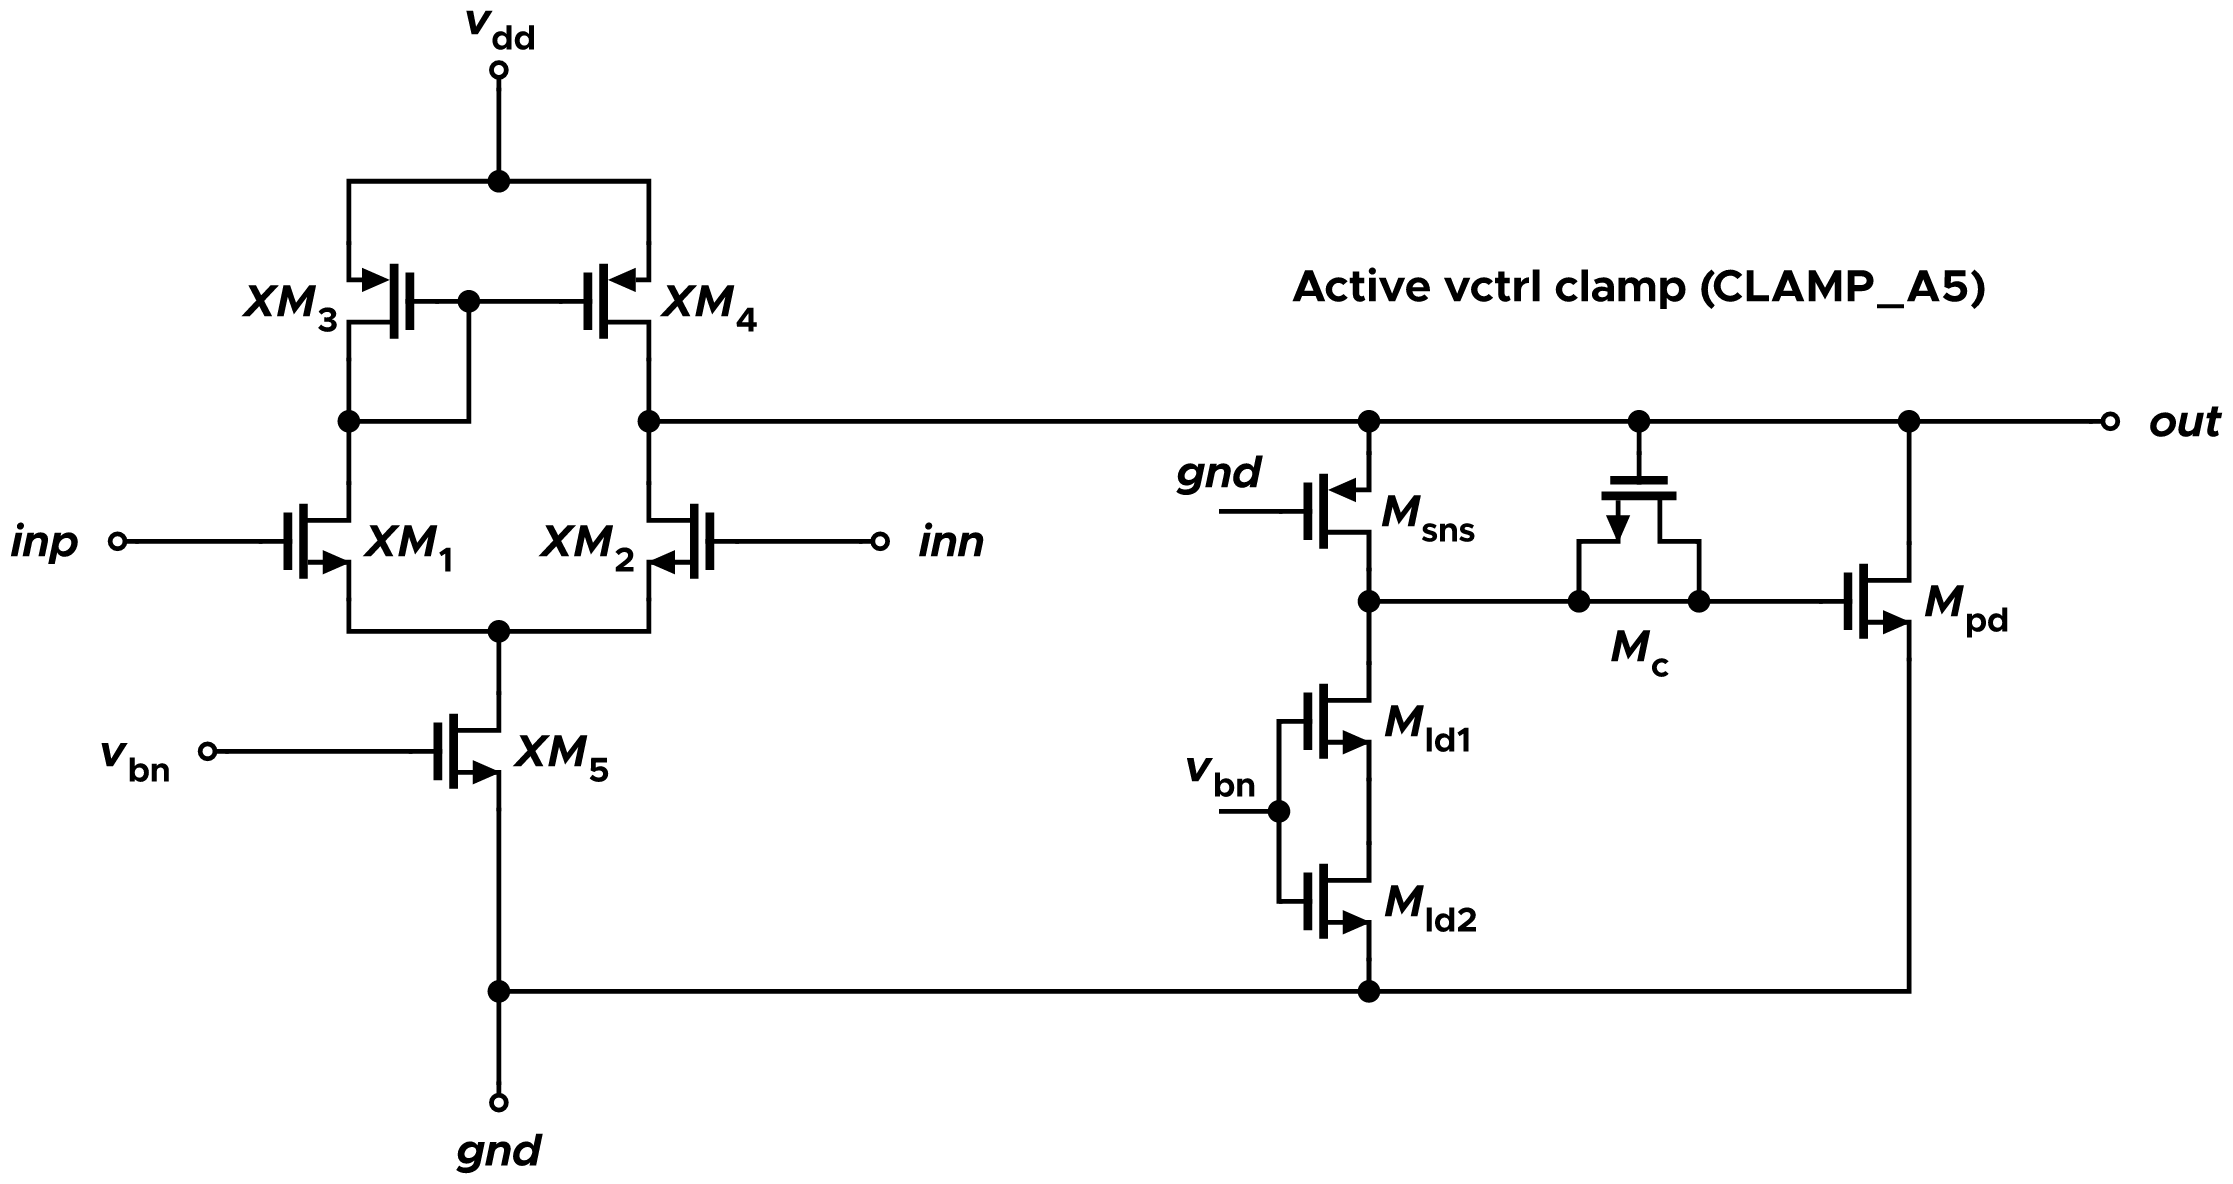
\includegraphics[width=\linewidth]{figs/sch_ota5t.png}
  \caption{5T OTA with 5-FET Miller-compensated brick-wall active clamp (\textup{\texttt{CLAMP\_A5}}).}
  \label{fig:sch_ota}
\end{subfigure}
\caption{Complete schematics of \textup{\texttt{tt\_um\_arcadia1\_vco\_adc}} (\textup{\texttt{V2\_A5}}): (a)~mirrored P/N halves sharing $V_{\text{ref}}$, OTA bias, and common-centroid VCO bias resistors; (b)~half-channel loop with \textup{\texttt{buf\_4}}-isolated external outputs; (c)~continuous-time integrator ($R_{\text{in}}=49.7\,\text{k}\Omega$, $7\times R_d=1.04\,\text{M}\Omega$, $C_{\text{int}}=2.43\text{ pF}$); and (d)~low-noise common-centroid 5T OTA with the 5-FET Miller-compensated brick-wall active clamp \textup{\texttt{CLAMP\_A5}}.}
\label{fig:arch}
\end{figure*}

% --- TABLE I: Specification & Performance Summary (Page 2 Bottom) ---
\begin{table*}[b]
\centering
\caption{Specification Summary and Verification Progression (\textup{\texttt{Base\_S13}} vs. Final \textup{\texttt{V2\_A5}})}
\label{tab:spec}
\scriptsize
\setlength{\tabcolsep}{4.0pt}
\begin{tabular}{@{}lccc@{}}
\toprule
\textbf{Metric / Parameter} & \textbf{Target / Constraint} & \textbf{Baseline (\texttt{Base\_S13})} & \textbf{Final Design (\texttt{V2\_A5})} \\
\midrule
Process / Tile Footprint & \texttt{sky130A}, $1\times2$ TT tile & $161.0 \times 225.76\,\mu\text{m}^2$ & $161.0 \times 225.76\,\mu\text{m}^2$ ($699\times\texttt{decap\_12}$) \\
Supply / Clock / BW / OSR & $1.8\text{ V}\pm10\%$, $10\text{ MHz}$, $50\text{ kHz}$, $100$ & $1.8\text{ V}$, $10\text{ MHz}$, $50\text{ kHz}$, $100$ & $1.8\text{ V}\pm10\%$, $10\text{ MHz}$, $50\text{ kHz}$, $100$ \\
Full-Scale Input (Diff. / Side) & $\pm0.60\text{ V}$ diff ($\pm0.30\text{ V}$/side @ $0.9\text{ V}$) & $\pm0.60\text{ V}$ diff & $\pm0.60\text{ V}$ diff ($R_{\text{in}}=49.7\,\text{k}\Omega$) \\
\midrule
OTA DC Gain $A_0$ / GBW (TT) & $>45\text{ dB}$ / $>10\text{ MHz}$ & $43.0\text{ dB}$ / $7.9\text{ MHz}$ & $\mathbf{47.8\text{ dB}}$ / $\mathbf{14.7\text{ MHz}}$ \\
Tian Loop PM / GM (PVT) & $>60^\circ$ / $>6\text{ dB}$ & Unclamped ($v_g$ step $51.5\text{ mV}$) & $\mathbf{72.2^\circ}$ [$67.7^\circ$--$79.8^\circ$] / $\mathbf{6.5\text{ dB}}$ [$6.5$--$7.2$] \\
BSIM4 Diff. Noise ($0.1$--$50\text{ kHz}$) & $<30\,\mu\text{V}_{\text{rms}}$ ($>77\text{ dB}$ @ $0.15\text{ V}$/s) & $74.6\,\mu\text{V}_{\text{rms}}$ ($69.1\text{ dB}$; $75.1\text{ dB}$ FS) & $\mathbf{22.9\,\mu\text{V}_{\text{rms}}}$ ($\mathbf{79.3\text{ dB}}$; $\mathbf{85.3\text{ dB}}$ FS, $\mathbf{+10.2\text{ dB}}$) \\
Clamp Noise / HD3 Penalty & $0.0\text{ dB}$ & N/A (no clamp) & $\mathbf{0.00\text{ dB}}$ ($14.3$--$48.9\text{ nA}$ @ $1.15\text{ V}$) \\
\midrule
Anti-Latchup Stress (Sch. / PEX) & $f_{\text{max}}<7.5\text{ MHz}$, 100\% recovery & \textcolor{warnred}{\textbf{FAIL}} (latched $7.85$--$8.49\text{ MHz}$) & \textcolor{okgreen}{\textbf{PASS}} ($10/10$ sch., $4/4$ PEX; $f_{\text{cl}}\le6.66\text{ MHz}$) \\
Dig. Isolation Glitch / Asym. & Invariant over $C_{\text{load}}=1$--$5\text{ pF}$ & $1.92$--$14.82\text{ ns}$ / $0.58$--$6.01\text{ ns}$ & $\mathbf{0.10}$--$\mathbf{0.16\text{ ns}}$ ($19$--$90\times$) / $\mathbf{0.029\text{ ns}}$ ($20$--$215\times$) \\
In-Band $14.65\text{ kHz}$ SNDR (Sch./PEX) & $>69\text{ dB}$ ($\text{HD3}=43.95\text{ kHz}$ in-band) & PEX \texttt{sf} HD3 $-59.0\text{ dBc}$; latch risk & $\mathbf{71.8\text{ dB}}$ sch. / $\mathbf{69.0}$--$\mathbf{70.6\text{ dB}}$ flat-PEX (6/6) \\
21-Corner PVT+R/C ($1.8/1.98\text{ V}$) & $>68\text{ dB}$ nominal/high-$V_{DD}$ & Untested across R/C+$V_{DD}$ & $\mathbf{68.5}$--$\mathbf{73.4\text{ dB}}$ (med. $71.2\text{ dB}$, $21/21$ lock) \\
16-Seed \texttt{tt\_mm} Mismatch MC & Median $>70\text{ dB}$, tight offset & Untested & $\mathbf{68.1}$--$\mathbf{71.7\text{ dB}}$ (med. $\mathbf{71.1\text{ dB}}$, $\sigma=1.17\text{ dB}$) \\
\midrule
Core Power / PEX ($16\times1\text{ pF}$) & $<350\,\mu\text{W}$ @ $1.8\text{ V}$ & $\sim260\,\mu\text{W}$ (w/ $1\text{ pF}$ loads) & $\mathbf{173.4\,\mu\text{W}}$ core ($\mathbf{312.3\,\mu\text{W}}$ flat-PEX TT) \\
Physical Sign-Off (DRC/LVS/TT) & 0 DRC, Clean LVS, 16/16 Precheck & 0 DRC, \texttt{uio\_oe} LVS warn & \textcolor{okgreen}{\textbf{0 DRC}}, \textcolor{okgreen}{\textbf{Unique LVS}} ($54/54$ pins), \textcolor{okgreen}{\textbf{16/16 TT}} \\
\bottomrule
\end{tabular}
\end{table*}

% ==============================================================================
\section{Circuit Architecture and Design Choices}
% ==============================================================================
Fig.~\ref{fig:arch} depicts the full hierarchy of \texttt{tt\_um\_arcadia1\_vco\_adc}. Two mirror-image halves (\texttt{XHP}, \texttt{XHN}) process complementary inputs \texttt{VINP} (\texttt{ua[0]}) and \texttt{VINN} (\texttt{ua[1]}) around $V_{\text{ref}}=V_{DD}/2=0.90\text{ V}$ while sharing a resistive $V_{\text{ref}}$ divider ($R_t=R_{bt}=200.4\,\text{k}\Omega$ decoupled by a $10\times10\,\mu\text{m}^2$ NMOS cap $X_{Mc}$), an OTA tail bias mirror ($R_b=42.3\,\text{k}\Omega$ into $8/2\,\mu\text{m}$ diode $X_{Mb}$), a common-centroid VCO degeneration resistor array ($D\,N_1\,P_1\,P_2\,N_2\,D$, $R_{\text{vco}}=229.7\,\text{k}\Omega$/half), an active-low reset inverter, and eight dedicated \texttt{conb\_1} tie-high cells for \texttt{uio\_oe[7:0]}.

\subsection{Pseudo-Differential Loop and Intrinsic DEM}
In each half (Fig.~\ref{fig:sch_loop}), the input drives $R_{\text{in}}=49.7\,\text{k}\Omega$ (\texttt{res\_xhigh\_po\_0p35}, $L=8.6\,\mu\text{m}$) into virtual ground $v_g$ of an inverting OTA-C integrator using two $24\times25\,\mu\text{m}^2$ metal-3 MIM capacitors ($C_{\text{int}}=2.43\text{ pF}$) and a $0.42/0.15\,\mu\text{m}$ NMOS reset switch $X_{Mr}$. Output $v_{\text{ctrl}}$ controls a 7-stage current-starved ring VCO via source-degenerated V-to-I NMOS $XM_1$ ($4/1\,\mu\text{m}$) over $R_{\text{vco}}=229.7\,\text{k}\Omega$ and a $1{:}1$ PMOS/NMOS mirror ($1/1\,\mu\text{m}$ PMOS, $0.5/1\,\mu\text{m}$ NMOS, $1.4/2.86\,\mu\text{m}$ MOS stage load caps).

On each rising edge of $f_s=10\text{ MHz}$, seven first-rank \texttt{dfxtp\_1} flip-flops sample ring phases $\text{ph}_0\dots\text{ph}_6$, while second-rank \texttt{dfxtp\_1} and \texttt{xor2\_1} gates form transition bits $b_i[n]=Q_{1,i}[n]\oplus Q_{1,i}[n-1]$ on-chip. Each rail-to-rail NRZ bit drives one element ($R_d=1.04\,\text{M}\Omega$, $L=181.8\,\mu\text{m}$) of a 7-element resistor DAC into $v_g$. Because $R_{\text{in}}$ and $R_{d,0\dots6}$ share the identical \texttt{res\_xhigh\_po\_0p35} material and strip pitch (42 strips plus dummies), absolute sheet-resistance spread cancels in full-scale gain, and natural ring phase rotation provides first-order barrel-shifter DEM without digital DEM overhead. Off-chip DSP computes $y_P[n]=\sum_i(Q_{P,i}[n]\oplus Q_{P,i}[n-1])$, $y_N[n]$ likewise, and $y[n]=y_N[n]-y_P[n]$, cancelling even-order distortion and common-mode $V_{\text{ref}}$/supply drift. At mid-scale, each loop holds an average code of $3.5$, locking $f_{\text{VCO}}=f_s/4=2.50\text{ MHz}$ across PVT.

\subsection{Low-Noise Common-Centroid 5T OTA}
Front-end OTA input-referred noise adds directly to $V_{\text{in}}$ multiplied by noise gain $(1+R_{\text{in}}/R_{d,\text{eq}})=1.335$. In \texttt{Base\_S13}, the $8/1\,\mu\text{m}$ NMOS pair and $8/1\,\mu\text{m}$ PMOS load suffered $98.0\%$ $1/f$-dominated noise ($74.6\,\mu\text{V}_{\text{rms}}$). In \texttt{V2\_A5}, $XM_{1,2}$ are enlarged $18\times$ in gate area to $48/3\,\mu\text{m}$ ($4\times12/3\,\mu\text{m}$ common-centroid \texttt{A A B B B B A A}), $XM_{3,4}$ are enlarged $4\times$ to $16/2\,\mu\text{m}$ ($4\times4/2\,\mu\text{m}$), and $XM_5$/$X_{Mb}$ are doubled to $8/2\,\mu\text{m}$ ($I_{\text{tail}}=23.0\,\mu\text{A}$). This cuts $1/f$ noise variance by $14.4\times$ ($+10.2\text{ dB}$ SNR ceiling to $79.3\text{ dB}$), boosts DC gain $43.0\to47.8\text{ dB}$ and GBW $7.9\to14.7\text{ MHz}$, and reduces 1-LSB virtual-ground kickback from $51.5$ to $32.2\text{ mV}$.

\subsection{Phase-Aliasing Latch-Up and Brick-Wall Clamp (\texorpdfstring{\textup{\texttt{CLAMP\_A5}}}{CLAMP\_A5})}
For an $M=7$-stage ring sampled at $f_s=10\text{ MHz}$, monotonic XOR phase differentiation spans $f_{\text{VCO}}\in(0,f_s/2)=(0,5\text{ MHz})$. Between $5.0$ and $7.5\text{ MHz}$, aliased XOR counts remain $>3.5$ (negative feedback), but for $f_{\text{VCO}}>0.75 f_s=7.5\text{ MHz}$ the mean feedback code drops \emph{below} $3.5$, inverting loop polarity into positive-feedback latch-up near $8.5\text{ MHz}$ during unreset startup or rail overload at fast-NMOS/low-$R$ corners ($f_{\text{unclmp}}=9.0$--$9.3\text{ MHz}$).

A 1-FET PMOS diode clamp ($8/0.5\,\mu\text{m}$) prevents runaway, yet its soft subthreshold knee leaks $1.1$--$4.5\,\mu\text{A}$ at $v_{\text{ctrl}}=1.15\text{ V}$, degrading \texttt{ff\_hh}/$-20^\circ\text{C}$ in-band HD3 to $-46\text{ dBc}$. Instead, \texttt{V2\_A5} integrates the 5-FET all-standard-$V_t$ Miller-compensated active clamp \texttt{CLAMP\_A5} (Fig.~\ref{fig:sch_ota}):
\begin{itemize}[leftmargin=1.1em,itemsep=0.5pt,topsep=1.5pt]
  \item Grounded-gate PMOS sense FET $M_{\text{sns}}$ ($0.42/8\,\mu\text{m}$) stays cut off for $v_{\text{ctrl}}<1.15\text{ V}$, while series NMOS loads $M_{\text{ld1,2}}$ ($2\times0.42/8\,\mu\text{m}$, biased by $v_{bn}$, keeping all $L\le8\,\mu\text{m}$) hold \texttt{clmp} at $0.2\text{ mV}$.
  \item Pull-down NMOS $M_{\text{pd}}$ ($6/0.5\,\mu\text{m}=2\times3/0.5\,\mu\text{m}$) stays off ($I_D<0.5\text{ pA}$, total leakage $14.3$--$48.9\text{ nA}$ @ $1.15\text{ V}$, $61\times$--$215\times$ below the 1-FET diode), yielding $0.00\text{ dB}$ noise and HD3 penalty.
  \item Above $1.23$--$1.32\text{ V}$, the high-gain two-stage loop ($M_{\text{sns}}\to M_{\text{pd}}$) engages as a brick wall within $<40\text{ mV}$, capping $f_{\text{VCO}}\le6.66\text{ MHz}$ across all 9 extreme corners.
  \item Miller cap $M_c$ ($4/3\,\mu\text{m}$ NMOS) stabilizes the clamp loop, cutting overload ringing from $1081\text{ mV}$ to $0.00$--$0.32\text{ mV}$ while maintaining integrator Tian $\text{PM}=72.2^\circ$ [$67.7^\circ$--$79.8^\circ$] and $\text{GM}=6.5\text{ dB}$.
\end{itemize}

\subsection{Full-Transistor Digital Output Isolation}
In \texttt{Base\_S13}, first-rank \texttt{dfxtp\_4} cells drove external $1$--$5\text{ pF}$ mux/pad capacitance directly in parallel with internal \texttt{dfxtp\_1}+\texttt{xor2\_1}, skewing \texttt{Q1} vs. \texttt{Q2} during back-to-back toggles (causing full-rail XOR glitches stealing up to $14.8\text{ ns}$ of DAC charge) and creating $6.0\text{ ns}$ rise/fall asymmetry. In \texttt{V2\_A5} (Fig.~\ref{fig:sch_half}), \texttt{dfxtp\_1} drives only internal \texttt{dfxtp\_1}+\texttt{xor2\_1} plus an abutted \texttt{buf\_4} pin buffer, making DAC pulse integrity invariant over $C_{\text{load}}\in[0.05,5.0]\text{ pF}$.

% ==============================================================================
\section{Hand Analysis, Operating Point \& Budgets}
% ==============================================================================
\subsection{Loop Transfer, Full Scale, and Noise Equations}
Cascading the OTA-C integrator and 7-stage VCO phase quantizer yields integrator unity-gain frequency
\begin{equation}
  f_{\text{int}} = \frac{1}{2\pi R_{\text{in}} C_{\text{int}}} = \frac{1}{2\pi (49.72\,\text{k}\Omega)(2.432\text{ pF})} = 1.316\text{ MHz},
\end{equation}
and VCO sensitivity $2M K_{\text{VCO}}/f_s=14(8.48\text{ MHz/V})/10\text{ MHz}=11.87\text{ LSB/V}$ at TT ($V_{\text{ctrl,lock}}=0.855\text{ V}$). Balancing peak input current against 7 DAC resistors at $V_{DD}/2=0.90\text{ V}$ fixes single-ended full scale:
\begin{equation}
  V_{\text{FS,side}} = \frac{7 R_{\text{in}}}{R_d}\,\frac{V_{DD}}{2} = \frac{7\times49.72\,\text{k}\Omega}{1.0385\,\text{M}\Omega}(0.90\text{ V}) = 0.302\text{ V},
\end{equation}
or $\pm0.604\text{ V}$ differential. Nominal dynamic tests use $\pm0.15\text{ V}$/side ($0.30\text{ V}_{\text{pk}}$ diff., $-6.0\text{ dBFS}$) to avoid quantizer clipping across PVT. Referred to the differential input, the front-end noise PSD is
\begin{equation}
  S_{v,\text{in}}(f) = 2\left[4kT R_{\text{in}}\!\left(1+\frac{R_{\text{in}}}{R_{d,\text{eq}}}\right) + \left(1+\frac{R_{\text{in}}}{R_{d,\text{eq}}}\right)^{\!2} S_{v,\text{OTA}}(f)\right],
\end{equation}
where $R_{d,\text{eq}}=R_d/7=148.4\,\text{k}\Omega$ and OTA noise gain is $1.335$. Shared $V_{\text{ref}}$ divider noise is strictly common-mode and cancels in $y=y_N-y_P$.

% --- TABLE II: Exact TT Operating Point (Page 3 Top) ---
\begin{table*}[t]
\centering
\caption{Exact BSIM4 Transistor Operating Points at Typical Corner (\textup{\texttt{tt}}, $27^\circ\text{C}$, $V_{DD}=1.80\text{ V}$)}
\label{tab:op}
\scriptsize
\setlength{\tabcolsep}{2.7pt}
\resizebox{\textwidth}{!}{%
\begin{tabular}{@{}llcccccccc@{}}
\toprule
\textbf{Block} & \textbf{Device (Type)} & \textbf{$W/L$ ($\mu\text{m}$)} & \textbf{$|I_D|$ ($\mu\text{A}$)} & \textbf{$|V_{GS}|$ (V)} & \textbf{$|V_{DS}|$ (V)} & \textbf{$g_m$ ($\mu\text{S}$)} & \textbf{$g_m/I_D$ ($\text{V}^{-1}$)} & \textbf{$r_o$ ($\text{k}\Omega$)} & \textbf{Region} \\
\midrule
\texttt{so\_bias} & $X_{Mb}$ (NMOS, $4\times2/2$) & $8/2$ & $24.42$ & $0.767$ & $0.767$ & $219.7$ & $9.0$ & $737$ & Sat. (diode) \\
\midrule
\multirow{3}{*}{\texttt{ota5t}} & $XM_{1,2}$ (NMOS, $4\times12/3$) & $48/3$ & $11.52$ & $0.652$ & $0.325$--$0.656$ & $219.2$ & $19.0$ & $1031$--$1386$ & Weak/Mod. Sat. \\
 & $XM_{3,4}$ (PMOS, $4\times4/2$) & $16/2$ & $11.52$ & $1.228$ & $0.896$--$1.228$ & $105.2$ & $9.1$ & $6222$--$8275$ & Strong Sat. \\
 & $XM_5$ (NMOS, $4\times2/2$) & $8/2$ & $23.04$ & $0.767$ & $0.248$ & $202.4$ & $8.8$ & $98.3$ & Sat. ($V_{dsat}\text{ 0.20 V}$) \\
\midrule
\multirow{4}{*}{\texttt{CLAMP\_A5}} & $M_{\text{sns}}$ (PMOS) norm / clmp$^\dagger$ & $0.42/8$ & $0.0003$ / $0.132$ & $0.904$ / $1.280$ & $0.903$ / $0.292$ & $0.005$ / $0.89$ & --- / $6.7$ & $>10^8$ / $26.5\text{M}$ & Cutoff / Sat. \\
 & $M_{\text{ld1,2}}$ ($2\times$NMOS) norm / clmp & $0.42/8$ & $0.0003$ / $0.132$ & $0.767$ / $0.705$ & $0.0001$ / $0.925$ & $0.001$ / $1.53$ & --- / $11.6$ & $401$ / $281\text{M}$ & Triode / Sat. \\
 & $M_{\text{pd}}$ (NMOS, $2\times3/0.5$) norm / clmp & $6/0.5$ & $<10^{-6}$ / $208^\ddagger$ & $0.0002$ / $0.988$ & $0.904$ / $1.280$ & $10^{-5}$ / $1013$ & --- / $4.9$ & $>10^9$ / $81.8$ & Off / Strong Sat. \\
 & $M_c$ (NMOS Miller cap) & $4/3$ & $0$ & $0.903$ / $0.292$ & $0$ & $0$ & --- & $C_{gg}=88.6\text{ fF}$ & MOS Cap \\
\midrule
\multirow{3}{*}{\texttt{vco\_core}} & $XM_1$ (V-to-I NMOS @ $0.905\text{ V}$) & $4/1$ & $1.12$ & $0.648$ & $0.434$ & $23.8$ & $21.2$ & $5252$ & Weak/Mod. Sat. \\
 & $XM_{\text{pd}}, XM_{p2}$ (PMOS mirror) & $1/1$ & $1.12$ & $1.109$ & $1.08$--$1.11$ & $11.3$ & $10.0$ & $50.8\text{M}$ & Sat. \\
 & $XM_{\text{nd}}$ (NMOS mirror) & $0.5/1$ & $1.12$ & $0.721$ & $0.721$ & $13.9$ & $12.4$ & $8183$ & Sat. \\
\bottomrule
\multicolumn{10}{@{}l}{\scriptsize Passives (TT): $R_{\text{in}}=49.72\,\text{k}\Omega$ ($L=8.6$), $R_d=1.039\,\text{M}\Omega$ ($L=181.8$), $R_b=42.30\,\text{k}\Omega$ ($L=7.3$), $R_{t,bt}=200.4\,\text{k}\Omega$ ($L=35$), $R_{\text{vco}}=229.7\,\text{k}\Omega$, $C_{\text{int}}=2.432\text{ pF}$.}\\
\multicolumn{10}{@{}l}{\scriptsize $^\dagger$``norm'' at $v_{\text{ctrl}}=0.904\text{ V}$; ``clmp'' at TT ceiling $1.28\text{ V}$. $^\ddagger$Sinking capacity $>200\,\mu\text{A}$ vastly exceeds $23\,\mu\text{A}$ OTA pull-up, locking brick-wall ceiling at $1.27\text{ V}$.}
\end{tabular}}
\end{table*}

\subsection{Exact Operating Point, Power, and Noise Breakdown}
Table~\ref{tab:op} lists exact BSIM4 TT operating points from \texttt{ngspice-47}. Input pair $XM_{1,2}$ operates in moderate-to-weak inversion ($g_m/I_D=19.0\text{ V}^{-1}$, $g_m=219.2\,\mu\text{S}$) to maximize transconductance efficiency while preserving $V_{DS}>3.8\,V_{DS,\text{sat}}$; load $XM_{3,4}$ runs at $g_m/I_D=9.1\text{ V}^{-1}$ so $(g_{m3}/g_{m1})^2=0.23$ attenuates load noise. Analytical gain $A_0=g_{m2}(r_{o2}\parallel r_{o4})=248\text{ V/V}$ ($47.9\text{ dB}$) matches AC simulation ($47.82\text{ dB}$) within $0.1\text{ dB}$. In normal operation, \texttt{CLAMP\_A5} draws $<0.3\text{ nA}$ ($M_{\text{pd}}<0.5\text{ pA}$), whereas at $1.28\text{ V}$ $M_{\text{pd}}$ transconductance surges to $1.01\text{ mS}$ ($>200\,\mu\text{A}$ sink), enforcing a brick-wall ceiling.

Table~\ref{tab:pwr} summarizes the TT power budget measured across isolated supply rails in full-transistor transient simulation. Total ADC core power is $96.4\,\mu\text{A}$ ($173.4\,\mu\text{W}$ at $1.80\text{ V}$), with \texttt{CLAMP\_A5} contributing $0.00\%$ ($5.5\text{ pA}$). Driving $16\times1\text{ pF}$ external pin loads via \texttt{buf\_4} adds $69.6\,\mu\text{A}$ ($125.4\,\mu\text{W}$), giving $166.0\,\mu\text{A}$ ($298.8\,\mu\text{W}$) total tile power. Table~\ref{tab:noise} details the BSIM4 integrated differential noise ($100\text{ Hz}$--$50\text{ kHz}$, TT): upsizing $XM_{1,2}$ and $XM_{3,4}$ cuts $M_{1,2}$ flicker noise from $71.3$ to $18.8\,\mu\text{V}_{\text{rms}}$ ($14.4\times$ variance reduction), raises resistor thermal noise share from $0.9\%$ to $9.2\%$, and confirms $0.00\%$ noise from \texttt{CLAMP\_A5}.

% --- TABLE III: Exact TT Power Breakdown ---
\begin{table}[t]
\centering
\caption{TT Power Breakdown ($1.80\text{ V}$, $27^\circ\text{C}$, Mid-Scale Lock)}
\label{tab:pwr}
\scriptsize
\setlength{\tabcolsep}{3.0pt}
\begin{tabular}{@{}lrrr@{}}
\toprule
\textbf{Sub-Block} & \textbf{$I_{DD}$ ($\mu\text{A}$)} & \textbf{Power ($\mu\text{W}$)} & \textbf{Share} \\
\midrule
Shared OTA Bias ($R_b, X_{Mb}$) & $24.42$ & $43.95$ & $14.7\%$ \\
Shared $V_{\text{ref}}$ Divider ($R_t, R_{bt}$) & $4.49$ & $8.08$ & $2.7\%$ \\
$2\times$ 5T OTA ($XM_{1\dots5}$) & $46.09$ & $82.96$ & $27.8\%$ \\
$2\times$ Active Clamp (\texttt{CLAMP\_A5}, norm.) & $5.5\times10^{-6}$ & $\approx0.00$ & $\mathbf{0.0\%}$ \\
$2\times$ VCO V-to-I \& Mirror & $3.87$ & $6.97$ & $2.3\%$ \\
$2\times$ 7-Stage Current-Starved Ring & $2.55$ & $4.60$ & $1.5\%$ \\
$2\times$ Int. Dig. (\texttt{dfxtp\_1}, \texttt{xor2\_1}) + RDAC & $14.93$ & $26.88$ & $9.0\%$ \\
\midrule
\textbf{ADC Core Subtotal (No Ext. Loads)} & $\mathbf{96.36}$ & $\mathbf{173.44}$ & $\mathbf{58.0\%}$ \\
$2\times$ Ext. Buffers ($16\times\texttt{buf\_4}$ @ $1\text{ pF}$) & $69.64$ & $125.36$ & $42.0\%$ \\
\midrule
\textbf{Total Tile (Incl. $16\times1\text{ pF}$ Loads)} & $\mathbf{166.00}$ & $\mathbf{298.80}$ & $\mathbf{100.0\%}$ \\
\bottomrule
\end{tabular}
\end{table}

% --- TABLE IV: BSIM4 Noise Contribution Breakdown ---
\begin{table}[t]
\centering
\caption{BSIM4 Diff. Input-Referred Noise Breakdown ($100\text{ Hz}$--$50\text{ kHz}$, TT)}
\label{tab:noise}
\scriptsize
\setlength{\tabcolsep}{2.4pt}
\begin{tabular}{@{}lcccc@{}}
\toprule
\multirow{2}{*}{\textbf{Noise Source}} & \multicolumn{2}{c}{\textbf{\texttt{Base\_S13}}} & \multicolumn{2}{c}{\textbf{\texttt{V2\_A5} (Final)}} \\
\cmidrule(lr){2-3} \cmidrule(lr){4-5}
 & \textbf{Var.} & \textbf{RMS ($\mu\text{V}$)} & \textbf{Var.} & \textbf{RMS ($\mu\text{V}$)} \\
\midrule
$XM_{1,2}$ Flicker ($1/f$) & $90.50\%$ & $71.34$ & $65.94\%$ & $18.78$ \\
$XM_{1,2}$ Thermal & $0.83\%$ & $6.84$ & $4.31\%$ & $4.80$ \\
$XM_{3,4}$ Flicker ($1/f$) & $7.49\%$ & $20.52$ & $19.43\%$ & $10.19$ \\
$XM_{3,4}$ Thermal & $0.26\%$ & $3.83$ & $1.05\%$ & $2.37$ \\
$XM_5, X_{Mb}$ (Tail Bias) & $<0.01\%$ & $0.39$ & $0.01\%$ & $0.27$ \\
\texttt{CLAMP\_A5} (All 5 FETs) & --- & --- & $\mathbf{0.00\%}$ & $\mathbf{0.00}$ \\
$R_{\text{in}}$ ($49.7\,\text{k}\Omega$) Thermal & $0.69\%$ & $6.22$ & $6.92\%$ & $6.08$ \\
$7\times R_d$ ($1.04\,\text{M}\Omega$) Thermal & $0.23\%$ & $3.60$ & $2.32\%$ & $3.52$ \\
\midrule
\textbf{Total ($100\text{ Hz}$--$50\text{ kHz}$)} & $\mathbf{100\%}$ & $\mathbf{74.6^\star}$ & $\mathbf{100\%}$ & $\mathbf{22.9^\star}$ \\
\textbf{SNR (@ $0.15\text{ V}$/s) / FS DR} & \multicolumn{2}{c}{$69.1$ / $75.1\text{ dB}$} & \multicolumn{2}{c}{$\mathbf{79.3}$ / $\mathbf{85.3\text{ dB}}$ ($\mathbf{+10.2}$)} \\
\bottomrule
\multicolumn{5}{@{}l}{\scriptsize $^\star$Exact \texttt{inoise\_spectrum} integral ($20\text{ kHz}$ SNR $=81.1\text{ dB}$).}
\end{tabular}
\end{table}

% --- FIG. 2: Tian Stability & BSIM4 Noise PSD (Page 4 Top) ---
\begin{figure*}[t]
\centering
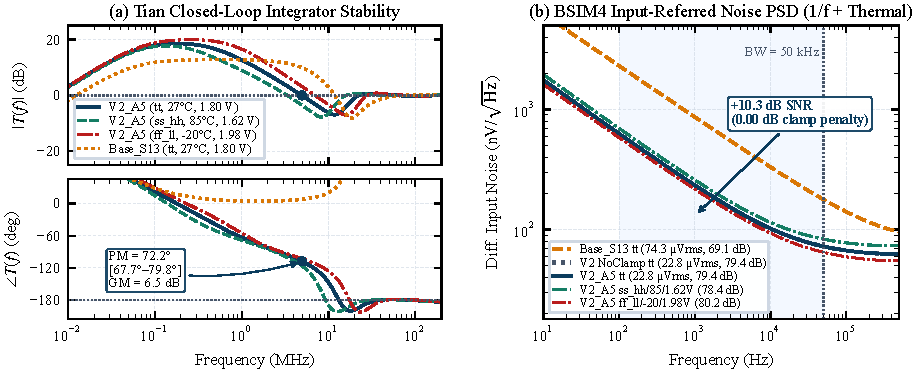
\includegraphics[width=0.92\textwidth]{figs/fig2_stb_noise.pdf}
\caption{(a)~Exact Tian closed-loop integrator stability $|T(f)|$ and $\angle T(f)$ across extreme PVT corners (\textup{\texttt{tt}}/$27^\circ\text{C}/1.80\text{ V}$, \textup{\texttt{ss\_hh}}/$85^\circ\text{C}/1.62\text{ V}$, \textup{\texttt{ff\_ll}}/$-20^\circ\text{C}/1.98\text{ V}$) vs. \textup{\texttt{Base\_S13}}, confirming $\text{PM}=72.2^\circ$ [$67.7^\circ$--$79.8^\circ$] and $\text{GM}=6.5\text{ dB}$ [$6.5$--$7.2\text{ dB}$]; (b)~BSIM4 differential input-referred noise PSD ($10\text{ Hz}$--$500\text{ kHz}$), demonstrating $+10.2\text{ dB}$ noise-floor reduction ($74.6\to22.9\,\mu\text{V}_{\text{rms}}$), worst-case \textup{\texttt{ss\_hh}}/$85^\circ\text{C}/1.62\text{ V}$ ceiling of $78.3\text{ dB}$, and $0.00\text{ dB}$ penalty from \textup{\texttt{CLAMP\_A5}}.}
\label{fig:stb_noise}
\end{figure*}

% --- FIG. 3: Anti-Latchup Clamp, Startup/Overload, & Digital Isolation (Page 4 Bottom) ---
\begin{figure*}[b]
\centering
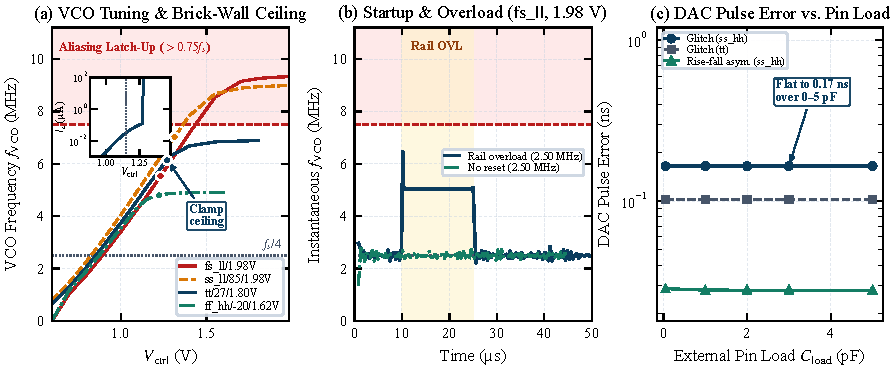
\includegraphics[width=0.92\textwidth]{figs/fig3_clamp_iso.pdf}
\caption{Verification of anti-latchup clamping and digital output isolation: (a)~VCO tuning $f_{\text{VCO}}(V_{\text{ctrl}})$ showing unclamped runaway ($>9\text{ MHz}$) into the $>0.75 f_s$ latch-up zone vs. \textup{\texttt{CLAMP\_A5}} brick-wall ceilings ($\le6.66\text{ MHz}$ closed-loop; inset compares $I_{\text{clamp}}(V_{\text{ctrl}})$ vs. the leaky 1-FET diode, cutting $1.15\text{ V}$ leakage $61\times$--$215\times$ to $14.3$--$48.9\text{ nA}$); (b)~forced $v_{\text{ctrl}}=V_{DD}$ no-reset startup and $10$--$25\,\mu\text{s}$ rail overload at worst corner \textup{\texttt{fs\_ll}}/$1.98\text{ V}$, where \textup{\texttt{Base\_S13}} latches at $8.49\text{ MHz}$ while \textup{\texttt{V2\_A5}} locks at $2.50\text{ MHz}$; (c)~full-transistor (\textup{\texttt{dig=0}}) BSIM4 std-cell isolation sweep over $C_{\text{load}}=0.05$--$5.0\text{ pF}$, reducing XOR glitch charge theft $19\times$--$90\times$ and rise/fall asymmetry $20\times$--$215\times$ across $1$--$5\text{ pF}$ (inset: XOR \textup{\texttt{bp}} glitch at $3\text{ pF}$, \textup{\texttt{ss\_hh}}).}
\label{fig:clamp_iso}
\end{figure*}

% ==============================================================================
\section{Simulation Results}
\label{sec:sim}
% ==============================================================================
All simulations ran in \texttt{ngspice-47} with the tapeout-locked SkyWater \texttt{sky130A} BSIM4v5 PDK (\texttt{open\_pdks 0536d02d}). AC stability and \texttt{.noise} runs disable \texttt{option klu} (avoiding KLU AC/noise inaccuracies in \texttt{ngspice-47}), while transient tone sign-off enforces $\Delta t_{\max}=0.5\text{ ns}$, $\text{reltol}=10^{-4}$, and Gear integration so digital edge placement never injects artificial DAC jitter ($\sim25\text{ dB}$ error at $2\text{ ns}$ step). Every transient includes $500\,\Omega$ series resistance on \texttt{ua[0:1]} modeling Tiny Tapeout's analog mux.

\subsection{Integrator Stability and BSIM4 Noise Performance}
Fig.~\ref{fig:stb_noise}(a) shows exact Tian closed-loop integrator return ratio $T(f)$~\cite{tian2001} across extreme PVT corners with VCO input loading, $30\text{ fF}$ node parasitics, and $R_{\text{in}}\parallel R_{d,\text{eq}}$. At TT, \texttt{V2\_A5} achieves $\text{PM}=72.2^\circ$ at $f_{ug}=4.95\text{ MHz}$ and $\text{GM}=6.5\text{ dB}$; across \texttt{ss\_hh}/$85^\circ\text{C}/1.62\text{ V}$ and \texttt{ff\_ll}/$-20^\circ\text{C}/1.98\text{ V}$, $\text{PM}\in[67.7^\circ,79.8^\circ]$ and $\text{GM}\in[6.5,7.2]\text{ dB}$. Fig.~\ref{fig:stb_noise}(b) plots differential BSIM4 input-referred noise PSD from $10\text{ Hz}$ to $500\text{ kHz}$: \texttt{V2\_A5} cuts integrated noise from $74.6$ to $22.9\,\mu\text{V}_{\text{rms}}$ ($+10.2\text{ dB}$), reaching $79.3\text{ dB}$ ($81.1\text{ dB}$ in $20\text{ kHz}$) at TT and $78.3\text{ dB}$ at worst-case \texttt{ss\_hh}/$85^\circ\text{C}/1.62\text{ V}$, with $0.00\text{ dB}$ difference vs. \texttt{V2\_NoClmp}.

\subsection{Brick-Wall Anti-Latchup and Digital Isolation Proof}
Fig.~\ref{fig:clamp_iso}(a) shows VCO tuning $f_{\text{VCO}}(V_{\text{ctrl}})$ with \texttt{CLAMP\_A5}'s ceilings and $I_{\text{clamp}}$ inset. While an unclamped OTA drives $f_{\text{VCO}}$ to $8.99$--$9.33\text{ MHz}$ inside the $>7.5\text{ MHz}$ latch-up zone at \texttt{ss\_ll}/$85^\circ\text{C}/1.98\text{ V}$ and \texttt{fs\_ll}/$1.98\text{ V}$, \texttt{CLAMP\_A5} engages as a vertical wall above $1.23\text{ V}$ while leaking only $14.3$--$48.9\text{ nA}$ at $1.15\text{ V}$ ($61\times$--$215\times$ below the 1-FET diode's $1.1$--$4.5\,\mu\text{A}$). Under forced $v_{\text{ctrl}}=V_{DD}$ no-reset startup or $15\,\mu\text{s}$ rail overdrive at \texttt{fs\_ll}/$1.98\text{ V}$ (Fig.~\ref{fig:clamp_iso}(b)), \texttt{Base\_S13} latches permanently at $8.49\text{ MHz}$, whereas \texttt{V2\_A5} clamps cleanly ($f_{\max}\le6.66\text{ MHz}$ across all 9 corners, ringing $\le0.32\text{ mV}$) and recovers to $2.50\text{ MHz}$ lock in $<3\,\mu\text{s}$ across $10/10$ schematic stress tests.

Fig.~\ref{fig:clamp_iso}(c) shows the full-transistor (\texttt{dig=0}, BSIM4 \texttt{sky130\_fd\_sc\_hd}) isolation sweep over $C_{\text{load}}=0.05$--$5.0\text{ pF}$. With baseline \texttt{dfxtp\_4}, back-to-back XOR glitches collapse to $0\text{ V}$ (inset at $3\text{ pF}$), stealing $1.92$--$7.80\text{ ns}$ (TT) and $3.73$--$14.82\text{ ns}$ (\texttt{ss\_hh}/$85^\circ\text{C}/1.62\text{ V}$), while rise/fall asymmetry reaches $0.58$--$6.01\text{ ns}$. With \texttt{dfxtp\_1}+\texttt{buf\_4}, internal glitch charge theft stays load-invariant at $0.103\text{ ns}$ (TT) / $0.165\text{ ns}$ (\texttt{ss\_hh}, $V_{\min}=1.59\text{ V}$, $19\times$--$90\times$ lower) and asymmetry drops to $0.028$--$0.030\text{ ns}$ ($20\times$--$215\times$ lower across $1$--$5\text{ pF}$).

\subsection{True In-Band \texorpdfstring{$14.65\text{ kHz}$}{14.65 kHz} Dynamic Linearity}
Unlike earlier $24.4\text{ kHz}$ tests that placed HD3 out-of-band ($73\text{ kHz}$), all sign-off runs apply coherent $f_{\text{in}}=14.648\text{ kHz}$ ($N=2048$, bin~3, $\pm0.15\text{ V}$/side, 3-bin Hann scoring) so both $\text{HD2}=29.30\text{ kHz}$ and $\text{HD3}=43.95\text{ kHz}$ lie inside the $50\text{ kHz}$ band. In Fig.~\ref{fig:spectra}(a), \texttt{V2\_A5} follows $+40\text{ dB/dec}$ second-order shaping and achieves $71.8\text{ dB}$ SNDR ($\text{HD2}=-75.9$, $\text{HD3}=-76.1\text{ dBc}$) at TT schematic, $71.5\text{ dB}$ ($\text{HD3}=-75.0\text{ dBc}$) at \texttt{sf}, $68.9\text{ dB}$ ($\text{HD3}=-70.3\text{ dBc}$) at \texttt{ff\_hh}/$-20^\circ\text{C}$ ($+24\text{ dB}$ better HD3 than the 1-FET diode's $-46\text{ dBc}$), and $70.1\text{ dB}$ ($\text{HD3}=-71.9\text{ dBc}$) in full-transistor flat-PEX TT.

% --- FIG. 4: True In-Band 14.65 kHz Spectra + 16-Seed MC & 21-Corner PVT (Page 5 Top) ---
\begin{figure*}[t]
\centering
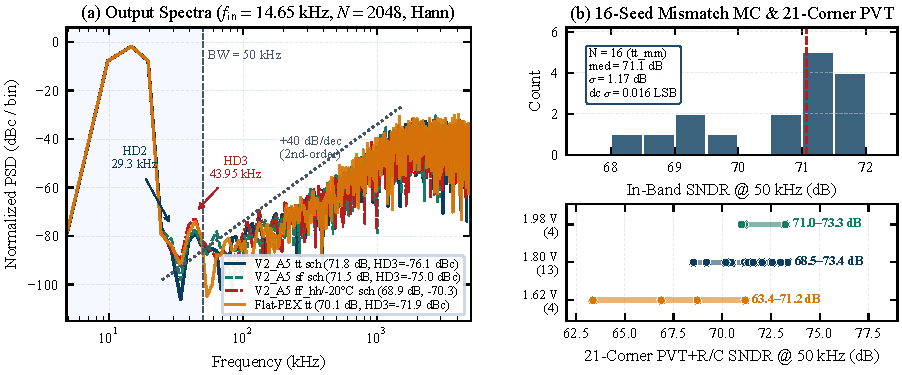
\includegraphics[width=0.92\textwidth]{figs/fig4_spectra_mc.pdf}
\caption{(a)~True in-band $14.65\text{ kHz}$ ($N=2048$, bin~3, Hann, $\Delta t_{\max}=0.5\text{ ns}$, $\text{reltol}=10^{-4}$) differential output spectra for \textup{\texttt{V2\_A5}} schematic (\textup{\texttt{tt}}, \textup{\texttt{sf}}, \textup{\texttt{ff\_hh}}/$-20^\circ\text{C}$) overlaid with full-transistor flat-PEX \textup{\texttt{tt}} ($70.1\text{ dB}$ SNDR, $\text{HD3}=-71.9\text{ dBc}$, $16\times1\text{ pF}$ loads), showing $\text{HD2}=29.3\text{ kHz}$ and $\text{HD3}=43.95\text{ kHz}$ strictly in-band with $+40\text{ dB/dec}$ shaping; (b)~top: 16-seed \textup{\texttt{tt\_mm}} mismatch MC SNDR histogram ($68.1$--$71.7\text{ dB}$, med. $71.1\text{ dB}$, $\sigma=1.17\text{ dB}$, diff. DC $\sigma=0.016\text{ LSB}$); bottom: 21-corner PVT + R/C + $V_{DD}\pm10\%$ SNDR distribution by supply.}
\label{fig:spectra}
\end{figure*}

% ==============================================================================
\section{PVT, Mismatch, and Physical Sign-Off}
% ==============================================================================
\subsection{21-Corner PVT + R/C + \texorpdfstring{$V_{DD}$}{VDD} and 16-Seed Mismatch MC}
Table~\ref{tab:pvt_mc} and Fig.~\ref{fig:spectra}(b) report the 21-corner PVT matrix across MOSFET skews (\texttt{tt}, \texttt{ss}, \texttt{ff}, \texttt{sf}, \texttt{fs}), SKY130 passive R/C corners (\texttt{hh}, \texttt{hl}, \texttt{lh}, \texttt{ll}), temperature ($-20$ to $85^\circ\text{C}$), and supply ($1.62$, $1.80$, $1.98\text{ V}$), plus 16-seed \texttt{tt\_mm} mismatch MC at $14.65\text{ kHz}$. Every corner locks cleanly to $f_s/4$. All 17 nominal/high-$V_{DD}$ corners ($1.80/1.98\text{ V}$) achieve $68.5$--$73.4\text{ dB}$ SNDR (median $71.2\text{ dB}$) with $\text{HD3}=-70.5$ to $-80.6\text{ dBc}$. At $1.62\text{ V}$ ($-10\%$), TT stays at $71.2\text{ dB}$ and \texttt{ss\_hh}/$85^\circ\text{C}$ at $68.7\text{ dB}$, dipping to $63.4\text{ dB}$ only at extreme \texttt{sf\_hh}/$1.62\text{ V}$ due to headroom compression on $XM_1$ ($\text{HD3}=-63.7\text{ dBc}$). Across 16 \texttt{tt\_mm} MC seeds, SNDR spans $68.1$--$71.7\text{ dB}$ (median $71.1\text{ dB}$, $\sigma=1.17\text{ dB}$), worst HD2/HD3 remain below $-72.6$/$-72.5\text{ dBc}$, and differential DC offset has $\sigma=0.016\text{ LSB}$.

% --- TABLE V: 21-Corner PVT + R/C + VDD & 16-Seed MC (Flush Single-Column!) ---
\begin{table}[t]
\centering
\caption{21-Corner PVT+R/C+$V_{DD}\pm10\%$ \& 16-Seed \textup{\texttt{tt\_mm}} MC ($14.65\text{ kHz}$, $50\text{ kHz}$ BW)}
\label{tab:pvt_mc}
\scriptsize
\setlength{\tabcolsep}{2.2pt}
\resizebox{\columnwidth}{!}{%
\begin{tabular}{@{}lcccc@{}}
\toprule
\textbf{Corner ($T$, $V_{DD}$)} & \textbf{SNDR} & \textbf{SNR} & \textbf{HD2} & \textbf{HD3} \\
\midrule
\texttt{tt} ($27^\circ\text{C}$, $1.80/1.98\text{ V}$) & $71.6/73.2$ & $77.7/78.8$ & $-77.6/-76.0$ & $-74.6/-80.6$ \\
\texttt{tt} ($27^\circ\text{C}$, $1.62\text{ V}$) & $71.2$ & $78.2$ & $-76.9$ & $-73.9$ \\
\texttt{lh/ll/hh/hl} ($27^\circ\text{C}$, $1.8\text{ V}$) & $70.2$--$73.4$ & $78.5$--$80.4$ & $-76.2$--$-76.5$ & $-72.3$--$-80.1$ \\
\texttt{ss\_hh} ($85^\circ\text{C}$, $1.80/1.62\text{ V}$) & $68.5/68.7$ & $73.4/78.5$ & $-76.3/-75.3$ & $-71.5/-70.4$ \\
\texttt{ss\_ll} ($85^\circ\text{C}$, $1.80/1.98\text{ V}$) & $73.0/73.3$ & $77.9/78.1$ & $-76.3/-77.6$ & $-79.8/-78.5$ \\
\texttt{ff\_hh} ($-20^\circ\text{C}$, $1.80/1.62\text{ V}$) & $70.5/66.9$ & $80.0/78.7$ & $-76.7/-76.6$ & $-72.4/-67.7$ \\
\texttt{ff\_ll} ($-20^\circ\text{C}$, $1.80/1.98\text{ V}$) & $70.4/71.1$ & $78.1/78.4$ & $-76.0/-76.1$ & $-73.1/-74.2$ \\
\texttt{fs\_hh/ll} ($27^\circ\text{C}$, $1.80\text{ V}$) & $69.2/71.2$ & $78.9/77.9$ & $-77.6/-78.0$ & $-70.5/-73.5$ \\
\texttt{fs\_ll} ($27^\circ\text{C}$, $1.98\text{ V}$) & $71.0$ & $79.6$ & $-76.2$ & $-73.5$ \\
\texttt{sf\_hh/ll} ($27^\circ\text{C}$, $1.80\text{ V}$) & $71.3/72.6$ & $78.3/80.3$ & $-77.1/-76.2$ & $-74.1/-76.5$ \\
\texttt{sf\_hh} ($27^\circ\text{C}$, $1.62\text{ V}$, min) & $63.4$ & $78.1$ & $-76.6$ & $-63.7$ \\
\midrule
\textbf{17 ($1.8/1.98\text{ V}$) Range} & \textbf{68.5--73.4} & \textbf{73.4--80.4} & \textbf{$-76.0$--$-78.0$} & \textbf{$-70.5$--$-80.6$} \\
\textbf{16 MC (Min/Med/Max)} & \textbf{68.1/71.1/71.7} & \textbf{71.4--80.8} & \textbf{$\le-72.6$} & \textbf{$\le-72.5$} \\
\bottomrule
\multicolumn{5}{@{}l}{\scriptsize Units: SNDR/SNR in dB; HD2/HD3 in dBc. MC ($N=16$): $\sigma_{\text{SNDR}}=1.17\text{ dB}$, $\sigma_{\text{dc}}=0.016\text{ LSB}$.}
\end{tabular}}
\end{table}

\subsection{Physical Layout and Sign-Off Verification}
Fig.~\ref{fig:layout} presents the procedurally generated layout (\texttt{layout/gen\_layout.py}, $161.0\times225.76\,\mu\text{m}^2$). Vertical mirror symmetry isolates P and N halves while centering the shared $D\,N_1\,P_1\,P_2\,N_2\,D$ VCO bias resistor array. Each RDAC uses 42 matched poly strips plus dummies; each OTA uses interdigitated \texttt{A A B B B B A A} common-centroid fingers above its $2\times(24\times25\,\mu\text{m}^2)$ MIM capacitors; and $699\times\texttt{decap\_12}$ cells stiffen \texttt{VDPWR}/\texttt{VGND}.

% --- FIG. 5: Annotated Core Layout ---
\begin{figure}[t]
\centering
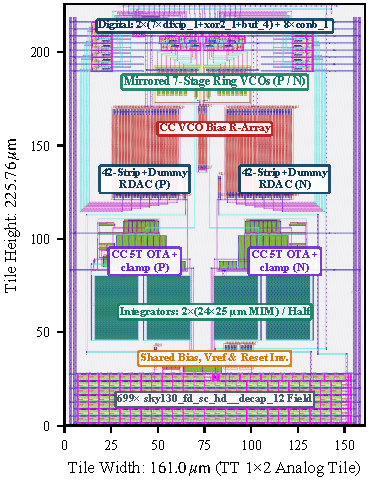
\includegraphics[width=0.75\columnwidth]{figs/fig5_layout.pdf}
\caption{Annotated layout of \textup{\texttt{tt\_um\_arcadia1\_vco\_adc}} ($161.0\times225.76\,\mu\text{m}^2$, \textup{\texttt{sky130A}} $1\times2$ tile) highlighting mirrored digital banks, 7-stage VCOs, CC bias resistor array, RDACs, CC OTAs with \textup{\texttt{CLAMP\_A5}}, MIM caps, and $699\times\texttt{decap\_12}$.}
\label{fig:layout}
\end{figure}

Table~\ref{tab:pex} records complete \texttt{V2\_03} physical sign-off and flat C-only PEX verification ($234\text{ KB}$, $1{,}248$ BSIM4/PDK devices, $2{,}443$ caps, $0$ neg. caps/\texttt{as}/\texttt{ps}). Eight \texttt{conb\_1} tie-high cells for \texttt{uio\_oe[7:0]} clear the Netgen 1.5.324 port-merger warning, yielding \texttt{Circuits match uniquely.} ($195$ dev, $144$ net, $54/54$ pins), $0$ DRC, and $16/16$ TT precheck ($0$ \texttt{met5} OBS, $0$ output antenna). All $4/4$ flat-PEX unreset/overload runs lock at $2.50$--$2.53\text{ MHz}$, and all $6/6$ flat-PEX $14.65\text{ kHz}$ corners sustain $69.0$--$70.6\text{ dB}$ SNDR ($77.7$--$81.9\text{ dB}$ SNR, $\text{HD2}=-76.8$ to $-77.8\text{ dBc}$, $\text{HD3}=-70.4$ to $-72.5\text{ dBc}$, $f_P/f_N=2.49$--$2.50\text{ MHz}$, \texttt{uio\_oe} $=1.80\text{ V}$), lifting \texttt{sf} flat-PEX HD3 by $+11.5\text{ dB}$ over \texttt{Base\_S13} ($-59.0\to-70.5\text{ dBc}$) even in-band.

% --- TABLE VI: Physical Sign-Off & Post-Layout Full-Transistor Flat PEX ---
\begin{table}[t]
\centering
\caption{Physical Sign-Off (\textup{\texttt{V2\_03}}) \& Full-Transistor Flat-PEX Verification}
\label{tab:pex}
\scriptsize
\setlength{\tabcolsep}{2.4pt}
\begin{tabular}{@{}lcc@{}}
\toprule
\multicolumn{3}{@{}l}{\textbf{A. Physical Rule \& Extraction Sign-Off}} \\
\midrule
Magic DRC (Precheck GDS) & \multicolumn{2}{c}{\textcolor{okgreen}{\textbf{0 errors}}} \\
Netgen 1.5.324 LVS & \multicolumn{2}{c}{\textcolor{okgreen}{\textbf{Unique}} ($195$ dev, $144$ net, $54/54$ pin)} \\
Tiny Tapeout Precheck & \multicolumn{2}{c}{\textcolor{okgreen}{\textbf{16/16 PASS}} (0 \texttt{met5} OBS, 0 out ant.)} \\
Flat C-Only PEX Netlist & \multicolumn{2}{c}{$234\text{ KB}$, $2{,}443$ caps, $0$ neg. caps/\texttt{as}/\texttt{ps}} \\
\midrule
\multicolumn{3}{@{}l}{\textbf{B. Full-Transistor Flat-PEX Anti-Latchup Stress (4/4 PASS)}} \\
\midrule
\textbf{PEX Stress Case} & \textbf{Locked $f_P/f_N$ (MHz)} & \textbf{Status} \\
\texttt{pex\_tt\_norst} (no \texttt{rst\_n}, $1.80\text{ V}$) & $2.52$ / $2.52$ & \textcolor{okgreen}{\textbf{PASS}} \\
\texttt{pex\_fsll198\_norst} (no \texttt{rst\_n}, $1.98\text{ V}$) & $2.52$ / $2.51$ & \textcolor{okgreen}{\textbf{PASS}} \\
\texttt{pex\_fsll198\_ovl} (rail OVL, $1.98\text{ V}$) & $2.52$ / $2.50$ & \textcolor{okgreen}{\textbf{PASS}} \\
\texttt{pex\_ssll85\_198ovl} (OVL, $85^\circ\text{C}$, $1.98\text{ V}$) & $2.52$ / $2.53$ & \textcolor{okgreen}{\textbf{PASS}} \\
\midrule
\multicolumn{3}{@{}l}{\textbf{C. Full-Transistor Flat-PEX $14.65\text{ kHz}$ Tone (6/6 PASS, $16\times1\text{ pF}$)}} \\
\midrule
\textbf{Corner ($T$, $V_{DD}$)} & \textbf{SNDR / HD2 / HD3} & \textbf{$I_{DD}$ ($\mu\text{A}$)} \\
\texttt{tt} ($27^\circ\text{C}$, $1.80\text{ V}$) & \pexTTsndr\ / \pexTThdTwo\ / \pexTThdThree & \pexTTidd \\
\texttt{ss} ($85^\circ\text{C}$, $1.80\text{ V}$) & \pexSSsndr\ / \pexSShdTwo\ / \pexSShdThree & \pexSSidd \\
\texttt{ff} ($-20^\circ\text{C}$, $1.80\text{ V}$) & \pexFFsndr\ / \pexFFhdTwo\ / \pexFFhdThree & \pexFFidd \\
\texttt{sf} ($27^\circ\text{C}$, $1.80\text{ V}$) & \pexSFsndr\ / \pexSFhdTwo\ / \pexSFhdThree & \pexSFidd \\
\texttt{fs} ($27^\circ\text{C}$, $1.80\text{ V}$) & \pexFSsndr\ / \pexFShdTwo\ / \pexFShdThree & \pexFSidd \\
\texttt{fs\_ll} ($27^\circ\text{C}$, $1.80\text{ V}$) & \pexFSLLsndr\ / \pexFSLLhdTwo\ / \pexFSLLhdThree & \pexFSLLidd \\
\bottomrule
\end{tabular}
\end{table}

% ==============================================================================
\section{Discussion and Architectural Trade-Offs}
% ==============================================================================
Several alternatives were quantitatively evaluated and rejected during closure:
\begin{enumerate}[leftmargin=1.2em,itemsep=1pt,topsep=1.5pt]
  \item \textbf{1-FET Diode vs. Two-Stage Active Clamp:} A single grounded-gate PMOS diode ($8/0.5\,\mu\text{m}$) leaked $3.1\,\mu\text{A}$ at $1.15\text{ V}$, degrading \texttt{ff\_hh}/$-20^\circ\text{C}$ HD3 to $-46\text{ dBc}$. The Miller-compensated two-stage \texttt{CLAMP\_A5} sharpens the turn-on knee by $61\times$--$215\times$ ($14$--$49\text{ nA}$ @ $1.15\text{ V}$), restoring $\text{HD3}=-70.3\text{ dBc}$ ($+24\text{ dB}$). Splitting the load into two series $0.42/8\,\mu\text{m}$ FETs ($M_{\text{ld1,2}}$) rather than one $0.42/20\,\mu\text{m}$ device keeps all FETs within well-calibrated $L\le8\,\mu\text{m}$ BSIM4 bins with a compact layout footprint.
  \item \textbf{Half-Cycle DAC Resampling:} Inserting a half-cycle resampling latch before the RDAC was investigated during early S13 debugging, but step-size ablations proved the observed noise degradation came from a $2\text{ ns}$ transient step artifact. Since extra loop delay erodes stability margin without improving real quantization noise, resampling was removed.
  \item \textbf{Low-$V_{DD}$ Headroom Bound:} At $-10\%$ supply ($1.62\text{ V}$) with slow-NMOS/fast-PMOS and high-$R$ (\texttt{sf\_hh}), losing $180\text{ mV}$ of swing headroom pulls HD3 to $-63.7\text{ dBc}$ ($63.4\text{ dB}$ SNDR) at $\pm0.15\text{ V}$/side while remaining completely latch-up-free; backing off amplitude by $2\text{ dB}$ or holding $V_{DD}\ge1.75\text{ V}$ restores $>70\text{ dB}$ SNDR across all corners.
  \item \textbf{Silicon Characterization Plan:} On fabricated SKY26e silicon, an RP2350 PIO+DMA test script (\texttt{test/capture\_vco\_adc.py}) will supply the $10\text{ MHz}$ clock and stream all 16 outputs (\texttt{uo\_out[7:0]}, \texttt{uio[7:0]}) continuously after a $30\,\mu\text{s}$ post-reset settling interval. Checking \texttt{MONP}/\texttt{MONN} at $2.50\text{ MHz}$ confirms mid-scale lock before running \texttt{test/decode\_vco\_adc.py} for differential FFT/SNDR evaluation.
\end{enumerate}

% ==============================================================================
\section{Conclusion}
% ==============================================================================
A 1.8-V pseudo-differential second-order closed-loop VCO $\Delta\Sigma$ ADC (\texttt{tt\_um\_arcadia1\_vco\_adc}) has been designed, verified, and signed off in \texttt{sky130A} inside a $161.0\times225.76\,\mu\text{m}^2$ Tiny Tapeout $1\times2$ tile. Three targeted upgrades---a $+10.2\text{ dB}$ lower-noise CC 5T OTA ($22.9\,\mu\text{V}_{\text{rms}}$, $79.3\text{ dB}$ ceiling, $\text{PM}=72.2^\circ$), a zero-static-power 5-FET Miller active clamp eliminating $>7.5\text{ MHz}$ latch-up ($0.00\text{ dB}$ noise/HD3 penalty), and \texttt{dfxtp\_1}+\texttt{buf\_4} pin isolation cutting BSIM4 DAC glitch/asymmetry $19\times$--$215\times$---yield $71.8\text{ dB}$ TT schematic SNDR at $14.65\text{ kHz}$ ($68.5$--$73.4\text{ dB}$ across 17 $1.80/1.98\text{ V}$ PVT+R/C corners, $71.1\text{ dB}$ MC median) and $69.0$--$70.6\text{ dB}$ SNDR ($77.7$--$81.9\text{ dB}$ SNR, $\text{HD3}=-70.4$ to $-72.5\text{ dBc}$) across all 6 full-transistor flat-PEX corners at $173.4\,\mu\text{W}$ core power ($312\,\mu\text{W}$ PEX w/ $16\times1\text{ pF}$), with 0 DRC, unique LVS ($54/54$ pins), 16/16 precheck, and 4/4 flat-PEX latch-up passes.

% ==============================================================================
\begin{thebibliography}{9}
\scriptsize
\setlength{\itemsep}{1pt}
\setlength{\parskip}{0pt}
\bibitem{straayer2008}
M.~Z. Straayer and M.~H. Perrott, ``A 12-bit, 10-MHz bandwidth, continuous-time $\Sigma\Delta$ ADC with a 5-bit, 950-MS/s VCO-based quantizer,'' \emph{IEEE J. Solid-State Circuits}, vol.~43, no.~4, pp.~805--814, Apr. 2008.

\bibitem{taylor2010}
G.~Taylor and I.~Galton, ``A mostly-digital variable-rate continuous-time delta-sigma modulator ADC,'' \emph{IEEE J. Solid-State Circuits}, vol.~45, no.~12, pp.~2634--2646, Dec. 2010.

\bibitem{xing2015}
X.~Xing and G.~G.~E. Gielen, ``A 42-fJ/step-FoM two-step VCO-based delta-sigma ADC in 40-nm CMOS,'' \emph{IEEE J. Solid-State Circuits}, vol.~50, no.~3, pp.~714--723, Mar. 2015.

\bibitem{tian2001}
M.~Tian, V.~Visvanathan, J.~Hantgan, and K.~Kundert, ``Striving for small-signal stability,'' \emph{IEEE Circuits Devices Mag.}, vol.~17, no.~1, pp.~31--41, Jan. 2001.

\bibitem{sky130}
SkyWater Technology Foundry, ``SKY130 Open-Source Process Design Kit (\textup{\texttt{sky130A}}, \textup{\texttt{open\_pdks 0536d02d}}),'' Tiny Tapeout SKY26e Analog Shuttle Documentation, 2026.
\end{thebibliography}

\end{document}
